% Bản thảo v3 tiếng Việt — bản dịch làm việc của paper/v3/manuscript_template.tex (bản tiếng Anh mới là bản nộp).
% Sinh bởi paper/v3/build.py từ các run đã xác minh accoding-learner-v3 và accoding-policy-v3;
% chỉ sửa tệp mẫu này hoặc các tệp trong sections/, không sửa manuscript_vi.tex.
\documentclass[a4paper,preprint,12pt,authoryear]{elsarticle}
\usepackage{amsmath,amssymb}
\usepackage{booktabs}
\usepackage{graphicx}
\usepackage[table]{xcolor}
\usepackage[hidelinks,hypertexnames=false]{hyperref}
\usepackage[capitalise,noabbrev]{cleveref}
\usepackage{microtype}
\usepackage{float}
\setlength{\emergencystretch}{3em}
\pdfpagewidth=\paperwidth \pdfpageheight=\paperheight % khổ A4
\newtheorem{proposition}{Mệnh đề}
\crefname{proposition}{Mệnh đề}{Mệnh đề}\Crefname{proposition}{Mệnh đề}{Mệnh đề}
\crefname{section}{Mục}{Mục}\Crefname{section}{Mục}{Mục}
\crefname{subsection}{Mục}{Mục}\Crefname{subsection}{Mục}{Mục}
\crefname{figure}{Hình}{Hình}\Crefname{figure}{Hình}{Hình}
\crefname{table}{Bảng}{Bảng}\Crefname{table}{Bảng}{Bảng}
\crefname{equation}{phương trình}{phương trình}\Crefname{equation}{Phương trình}{Phương trình}
\renewcommand{\appendixname}{Phụ lục}
\abstracttitle{Tóm tắt}
\keywordtitle{Từ khóa}
\AtBeginDocument{\renewcommand{\figurename}{Hình}\renewcommand{\tablename}{Bảng}\renewcommand{\refname}{Tài liệu tham khảo}}
\makeatletter
\g@addto@macro\appendix{\@addtoreset{table}{section}\@addtoreset{figure}{section}}
\makeatother
\myfooter[L]{Bản dịch tiếng Việt — không dùng để nộp tạp chí\hfill ngày 28 tháng 9 năm 2026}

\begin{document}
\begin{frontmatter}

\title{Bộ mô phỏng truy vết tri thức có thưởng cho việc học? Kiểm định bằng đối chứng âm cho gợi ý bài tập lập trình bằng học tăng cường}

\begin{abstract}
Các tác tử học tăng cường (RL) chọn bài tập lập trình thường được huấn luyện và đánh giá bên trong một mô hình truy vết tri thức (knowledge tracing, KT) fit từ log người học, và chính mô hình đó cũng đo lợi ích của tác tử. Chúng tôi kiểm định cách làm này trên 562.912 lần nộp đầu của 4.634 người học trên một hệ thống chấm bài lập trình C trực tuyến; không người học nào trong số đó được dùng trước khi các protocol nghiên cứu được khóa. Sáu mô hình người học, gồm truy vết tri thức sâu (DKT), dự báo người học chưa thấy tốt ngang nhau (AUC 0{,}775--0{,}776), và một cây định danh dựa trên entropy cho chẩn đoán đọc được. Các tác tử DQN và PPO huấn luyện với phần thưởng DKT vượt chọn ngẫu nhiên 13{,}2 và 27{,}2 điểm phần trăm xác suất làm đúng bài kiểm tra cuối kỳ vọng trong chính bộ mô phỏng huấn luyện, nhưng chỉ tối đa 0{,}35 điểm trong các thế giới fit độc lập có quá trình học ẩn tường minh. Trong một thế giới đối chứng âm, nơi việc học là không thể, tracker DKT vẫn báo tiến bộ 12{,}8 và 25{,}7 điểm cho các tác tử này, và trên 14 chính sách, tiến bộ trong mô phỏng tương quan thứ hạng gần như hoàn hảo với tiến bộ ảo đó (Spearman 0{,}960). Chúng tôi chứng minh rằng tiến bộ kỳ vọng của một chính sách bên trong bộ mô phỏng KT bằng tổng thay đổi mà mô hình tự dự đoán cho chính nó (độ trôi), và độ trôi bằng 0 với mô hình Bayes nhất quán không có học; độ trôi của DKT phân tán theo bài gấp 16 lần so với mô hình nhân tố cộng và ít được tái lập bởi một DKT huấn luyện lại với seed khác. Tác tử huấn luyện trong thế giới có cơ chế học tường minh theo số lần luyện chuyển giao tốt nhất giữa các thế giới ẩn cùng họ, nhưng không sang các thế giới nơ-ron. Chúng tôi khuyến nghị thế giới đối chứng âm, báo cáo độ trôi và các thế giới fit độc lập như những kiểm tra chuẩn cho đánh giá dựa trên mô phỏng của hệ gợi ý thích ứng.
\end{abstract}

\begin{keyword}
truy vết tri thức \sep học tăng cường \sep gợi ý bài tập \sep giáo dục lập trình \sep đánh giá dựa trên mô phỏng \sep đối chứng âm
\end{keyword}

\end{frontmatter}

\section{Giới thiệu}\label{sec:intro}

Các môn lập trình giao rất nhiều bài tập nhỏ, và người học tiến bộ với tốc độ rất khác nhau. Một bài quá khó làm người học nản lòng; một bài quá dễ dạy được rất ít. Gợi ý bài tập thích ứng giải quyết vấn đề này bằng cách ước lượng trạng thái của từng người học từ các lần làm trước và chọn bài tiếp theo cho phù hợp — một ý tưởng thường được gắn với vùng phát triển gần \citep{vygotsky1978mind} và có truyền thống lâu dài trong các hệ thống giáo dục thích ứng cho lập trình \citep{brusilovsky2007user,hsiao2010guiding}. Một công thức nay đã phổ biến kết hợp mô hình truy vết tri thức (knowledge tracing, KT), vốn dự báo khả năng người học làm đúng mỗi bài từ lịch sử của họ, với một tác tử học tăng cường (reinforcement learning, RL) coi việc chọn bài là một bài toán quyết định tuần tự: trạng thái của mô hình người học là trạng thái của tác tử, gợi ý một bài là một hành động, và mức tăng tri thức mà mô hình dự đoán là phần thưởng \citep{huang2019dre,liu2019cseal,ai2019cdkt,chen2023src,li2023gehrl,ozyurt2025exrec}. Vì thử nghiệm với người học tốn kém, các tác tử như vậy thường được huấn luyện \emph{và đánh giá} ngay bên trong mô hình người học đã fit, và mức tăng tri thức dự đoán được báo cáo như lợi ích của chính sách \citep{cheng2026unier}.

Cách đánh giá này chỉ tốt bằng mức bộ mô phỏng mô tả đúng việc luyện tập làm thay đổi khả năng làm đúng các bài khác như thế nào. Mô hình KT được fit và kiểm định trên dự báo bước kế tiếp của những chuỗi mà người học đã thực sự đi qua. Một chính sách, ngược lại, tạo ra chuỗi mới, và bộ mô phỏng phải ngoại suy hệ quả của các chuỗi đó. Hai mô hình có thể dự báo dữ liệu quan sát tốt như nhau mà vẫn bất đồng về những phản thực tế (counterfactual) như vậy \citep{breiman2001two,damour2022underspecification}. Với các quyết định dạy học, điều này đã được nhận ra từ sớm: tham số truy vết tri thức cá nhân hóa và tham số chung cho cả quần thể hàm ý lượng luyện tập rất khác nhau \citep{lee2012individualizing}, và các mô hình người học có độ chính xác dự báo tương tự có thể đề xuất lượng luyện tập khác nhau đáng kể \citep{rollinson2015predictive}. Ma trận đánh giá bền vững vì thế đánh giá mỗi chính sách ứng viên dưới nhiều mô hình người học \citep{doroudi2017rem}, và một tổng quan về RL cho sắp xếp trình tự dạy học nhận thấy các chính sách rút ra từ mô hình thuần dữ liệu thường không vượt được các đường cơ sở hợp lý khi thử với học sinh \citep{doroudi2019reward}. Trong học tăng cường nói chung, một bộ tối ưu được huấn luyện trên một mô hình hay một phần thưởng học từ dữ liệu sẽ khai thác chính sai số của mô hình đó \citep{kurutach2018metrpo,janner2019trust,gao2023scaling}. Các pipeline KT--RL hiện đại gộp cả hai rủi ro — mô hình học từ dữ liệu đồng thời là môi trường, phần thưởng và thước đo — nhưng hiếm khi có ai định lượng xem bao nhiêu phần của tiến bộ được báo cáo phản ánh việc học mà bộ mô phỏng mã hóa, và bao nhiêu phản ánh các đặc điểm riêng của bộ mô phỏng.

Chúng tôi nghiên cứu câu hỏi này cho lập trình nhập môn, dùng 1.291.558 lượt nộp C/C++ đã được chấm của 4.634 người học trên hệ thống chấm bài trực tuyến ACcoding \citep{chen2024accoding}. Chúng tôi fit sáu mô hình người học có độ chính xác dự báo ngang nhau, gồm DKT (truy vết tri thức sâu) làm tracker triển khai và một cây định danh dựa trên entropy để chẩn đoán dễ hiểu; huấn luyện các bộ gợi ý Double DQN và PPO trong ba loại thế giới huấn luyện; và đánh giá mọi chính sách trong chín thế giới khác nhau về tập người học được dùng để fit và về cách biểu diễn việc học. Hai công cụ làm cho việc đánh giá có tính chẩn đoán. Một thế giới \emph{đối chứng âm} không có bất kỳ việc học nào, trong đó tiến bộ thật của mọi chính sách đúng bằng 0, phơi bày trực tiếp các tiến bộ giả. Một \emph{phân rã} chính xác tiến bộ mà tracker báo cáo thành thay đổi dự báo mà mô hình tự kỳ vọng (\emph{độ trôi}) và \emph{phần bất ngờ} của bằng chứng cho thấy tiến bộ đó đến từ đâu. Chúng tôi chứng minh rằng độ trôi triệt tiêu với mô hình Bayes nhất quán không có học, và rằng bên trong chính bộ mô phỏng của nó, tiến bộ kỳ vọng của mọi chính sách bằng độ trôi mà chính sách tích lũy; do đó đánh giá trong mô phỏng thưởng cho chính sách vì đã chọn những bài mà mô hình \emph{kỳ vọng} sẽ nâng dự báo của chính nó.

Chúng tôi trả lời bốn câu hỏi nghiên cứu. RQ1: Các mô hình trạng thái nhận thức dự báo khả năng làm đúng ở lần nộp đầu của người học lập trình chưa thấy tốt đến đâu, và chúng có khác nhau không? RQ2: Tiến bộ của các bộ gợi ý RL lớn đến đâu trong bộ mô phỏng KT mà chúng được huấn luyện? RQ3: Các tiến bộ đó có đứng vững trong các thế giới fit độc lập không, và tracker báo tiến bộ bao nhiêu khi việc học là không thể? RQ4: Điều gì tạo ra sự chênh lệch, và chính sách nào vẫn bền vững? Tất cả protocol, gồm bốn giả thuyết, đã được khóa trên một cohort phát triển trước khi nạp quần thể đánh giá.

Đóng góp của bài báo gồm: (1) một pipeline đầu-cuối, có thể tái lập, cho gợi ý bài tập lập trình thích ứng trên dữ liệu thật, từ mô hình người học đến các tác tử DQN và PPO đã huấn luyện và một ứng dụng tương tác, với các giả thuyết đăng ký trước được kiểm định trên một quần thể chưa từng dùng; (2) bằng chứng rằng dù sáu mô hình người học dự báo tốt ngang nhau, tiến bộ trong mô phỏng của các tác tử thưởng theo KT co lại gần 0 trong các thế giới fit độc lập có học ẩn, và tương quan thứ hạng gần như hoàn hảo với tiến bộ mà tracker báo cáo trong một thế giới không có học; (3) phép phân rã độ trôi cùng hai mệnh đề giải thích các tiến bộ đó là thay đổi tự dự đoán tích lũy của tracker chứ không phải việc học — một chẩn đoán nội tại của mô hình, không cần thêm dữ liệu; và (4) bằng chứng thăm dò rằng tác tử huấn luyện trong thế giới có cấu trúc học tường minh chuyển giao tốt nhất giữa các thế giới ẩn cùng họ — nhưng không sang các thế giới nơ-ron — cùng các kiểm tra ít tốn kém cho đánh giá dựa trên mô phỏng.

\Cref{sec:related} điểm lại các nghiên cứu liên quan, \cref{sec:data} mô tả dữ liệu và \cref{sec:methods} trình bày các mô hình, bài toán quyết định, các thế giới đánh giá và phương pháp phân tích. \Cref{sec:results} báo cáo kết quả, \cref{sec:discussion} thảo luận hàm ý và giới hạn, và \cref{sec:conclusion} kết luận.

\section{Các nghiên cứu liên quan}\label{sec:related}

\subsection{Mô hình người học và truy vết tri thức}

Truy vết tri thức ước lượng tri thức đang thay đổi của người học từ chuỗi câu trả lời. Truy vết tri thức Bayes mô hình hóa mỗi thành phần tri thức như một trạng thái nhị phân ẩn \citep{corbett1994bkt}; các mô hình logistic như mô hình nhân tố cộng (additive factor model, AFM) và phân tích nhân tố thành tích (performance factors analysis, PFA) kết hợp năng lực người học, độ khó của bài và số lần luyện tập theo từng thành phần tri thức \citep{cen2006lfa,pavlik2009pfa,pelanek2017learner}, theo nghĩa thành phần tri thức mà \citet{koedinger2012kli} mô tả. Các mô hình hồi quy và mô hình dựa trên cơ chế chú ý, khởi đầu với DKT \citep{piech2015dkt} rồi SAKT và AKT \citep{pandey2019sakt,ghosh2020akt}, học động học trực tiếp từ dữ liệu \citep[xem tổng quan của][]{abdelrahman2023survey}. Nhiều so sánh cho thấy các mô hình logistic được đặc tả tốt đạt hoặc tiệm cận độ chính xác dự báo của mô hình sâu \citep{khajah2016deep,wilson2016basics,gervet2020deep}. Dự báo từng bước của DKT cũng có thể dịch chuyển theo hướng phi lý, chẳng hạn hạ mức thành thạo dự báo của một kỹ năng sau một câu trả lời đúng \citep{yeung2018dktplus}, dẫn tới các ràng buộc nhất quán và đơn điệu \citep{zhang2023cmkt}. Với lập trình, KT đã được mở rộng bằng đặc trưng mã nguồn \citep{shi2022codedkt}, và hỗ trợ điều hướng thích ứng từ lâu đã dẫn người học tới các bài lập trình có độ khó phù hợp \citep{hsiao2010guiding,brusilovsky2007user}. Dù vậy, việc đánh giá mô hình người học vẫn bị chi phối bởi độ chính xác dự báo trên dữ liệu giữ lại, mặc dù đã có những khung đánh giá mô hình qua hệ quả của nó đối với các quyết định dạy học \citep{gonzalezbrenes2015leopard,huang2015multifaceted}.

\subsection{Học tăng cường cho sắp xếp trình tự dạy học và gợi ý bài tập}

Sắp xếp trình tự dạy học bằng RL có lịch sử lâu dài. Các chính sách rút ra từ dữ liệu đã được thử với học sinh trong hệ thống dạy kèm thông minh \citep{chi2011umuai,shen2018jedm,zhou2022hrl}, trong khóa học trực tuyến \citep{bassen2020chi} và trong một hệ dạy toán dạng câu chuyện \citep{ruan2024rltutor}; các hướng liên quan dùng lập kế hoạch POMDP \citep{rafferty2016pomdp}, bandit nhiều cần gạt \citep{clement2015bandits} và mô hình dạy học xấp xỉ tối ưu \citep{whitehill2018teaching}. Các tổng quan kết luận rằng thành công là có thật nhưng không đồng đều: \citet{doroudi2019reward} nhận thấy chính sách rút ra từ mô hình người học thuần dữ liệu thường không vượt các đường cơ sở hợp lý khi thử với học sinh, và thành công dễ đạt hơn khi chính sách dựa trên mô hình có cơ sở lý thuyết; các tổng quan gần đây hơn chỉ ra các vấn đề phương pháp luận và nhu cầu đánh giá quy mô lớn hơn với người học thật \citep{singla2021rleducation,riedmann2025rlreview}. Song song, cộng đồng hệ gợi ý đã xây dựng các bộ gợi ý bài tập và lộ trình học bằng RL sâu, dựa vào một mô hình người học đã fit — thường là mô hình KT — để cung cấp trạng thái, phần thưởng hoặc thước đo việc học: gợi ý bài tập đa mục tiêu \citep{huang2019dre}, lộ trình học có nhận biết cấu trúc nhận thức \citep{liu2019cseal}, gợi ý dựa trên DKT có nhận biết khái niệm \citep{ai2019cdkt}, các bộ lập lộ trình dạng tập-thành-chuỗi và phân cấp \citep{chen2023src,li2023gehrl}, chưng cất trạng thái tri thức \citep{li2024pksd}, và ExRec, định nghĩa phần thưởng và điểm nhiệm vụ qua các trạng thái KT đã hiệu chỉnh \citep{ozyurt2025exrec}. Benchmark UniER hợp nhất các bộ gợi ý mức bài và mức lộ trình dưới một chỉ số tiến bộ nhận thức có trọng số rút từ KT \citep{cheng2026unier}, và các hệ lộ trình học bằng RL sâu cũng đã xuất hiện trên tạp chí này \citep{ruan2025adaptive}. Các công trình đó cải tiến biểu diễn và tối ưu hóa; câu hỏi của chúng tôi là bao nhiêu phần của một tiến bộ đo bằng KT còn đứng vững khi thế giới sinh ra kết quả không phải là mô hình đo kết quả.

\subsection{Từ độ chính xác dự báo đến quyết định dạy học}

Việc độ chính xác dự báo không quyết định được các lựa chọn dạy học là một phát hiện lặp lại. Với một tỉ lệ đáng kể học sinh, tham số truy vết tri thức chung của quần thể hàm ý lượng luyện tập khoảng gấp đôi so với tham số fit riêng cho từng người \citep{lee2012individualizing}; các mô hình người học có độ chính xác dự báo tương tự có thể hàm ý lượng luyện tập khác nhau đáng kể \citep{rollinson2015predictive}; tham số truy vết tri thức có thể suy biến về mặt ngữ nghĩa dù mô hình fit tốt \citep{doroudi2017identifiability}; và mô hình đặc tả sai có thể khiến quyết định về mức thành thạo thiếu công bằng giữa người học \citep{doroudi2019fairer}. \citet{gonzalezbrenes2015leopard} đề xuất đánh giá mô hình người học qua các quyết định dạy học mà nó tạo ra. Ma trận đánh giá bền vững \citep{doroudi2017rem} đánh giá mỗi chính sách ứng viên dưới nhiều mô hình người học và cảnh báo việc tin vào một chính sách chỉ tốt dưới chính mô hình đã sinh ra nó. Các bộ ước lượng off-policy dựa trên lấy mẫu theo trọng số quan trọng (importance sampling) đánh giá chính sách từ log mà không cần bộ mô phỏng \citep{mandel2014offline,thomas2016dataefficient}, nhưng chúng đòi hỏi xác suất hành động được ghi lại, điều mà việc tự luyện tập trên hệ thống chấm bài không cung cấp, nên mô phỏng vẫn là cách mặc định để đánh giá bộ gợi ý bài tập. Trong học máy nói chung, các bộ dự báo có độ chính xác tương đương trên dữ liệu giữ lại có thể hành xử rất khác nhau khi dùng cho tác vụ hạ nguồn \citep{breiman2001two,damour2022underspecification}.

\subsection{Tối ưu trên mô hình học từ dữ liệu và phần thưởng đại diện}

Trong RL dựa trên mô hình, một chính sách tối ưu trong mô hình động học học từ dữ liệu sẽ khai thác sai số của mô hình, nhất là ở vùng thiếu dữ liệu; các kỹ thuật tổ hợp mô hình (ensemble), mô phỏng ngắn và phạt độ bất định được đưa ra để hạn chế điều này \citep{kurutach2018metrpo,janner2019trust,yu2020mopo,moerland2023mbrl,levine2020offline}. Tương tự, tối ưu một mục tiêu đại diện có thể làm tăng mục tiêu đại diện trong khi mục tiêu thật đứng yên — hiện tượng lách hay chơi gian phần thưởng (reward hacking/gaming) \citep{amodei2016concrete,skalse2022reward} — và việc tối ưu quá mức một mô hình phần thưởng học từ dữ liệu tuân theo các quy luật co giãn dự đoán được \citep{gao2023scaling}. Bộ mô phỏng của hệ gợi ý thừa hưởng thiên lệch của log dùng để fit nó \citep{huang2020keeping}, và đánh giá ngoại tuyến là một trở ngại đã được thừa nhận khi triển khai RL trong thế giới thực \citep{dulacarnold2021challenges}. Bộ gợi ý KT--RL nằm ở giao điểm của các vấn đề này vì một mô hình học từ dữ liệu đóng cùng lúc vai trò động học, phần thưởng và thước đo đánh giá. Từ dịch tễ học, chúng tôi mượn khái niệm đối chứng âm: một phân tích mà hiệu ứng thật được biết chắc là không tồn tại, nên mọi hiệu ứng ước lượng được đều bộc lộ sai lệch \citep{lipsitch2010negative,arnold2016negative}.

Công trình này nối các mạch nghiên cứu trên cho bài toán gợi ý bài tập lập trình. Chúng tôi fit sáu mô hình người học có chất lượng dự báo ngang nhau trên cùng dữ liệu thật và cho thấy sự bất đồng giữa chúng lan truyền sang thứ hạng chính sách như thế nào, đồng thời bổ sung hai công cụ mà các nghiên cứu về đánh giá bền vững chưa dùng: một thế giới đối chứng âm không có học, trong đó tiến bộ thật của mọi chính sách đúng bằng 0, và một phép phân rã chính xác tiến bộ mà tracker báo cáo thành độ trôi và phần bất ngờ, kèm các kết quả hình thức đồng nhất tiến bộ trong mô phỏng với độ trôi tích lũy.

\section{Dữ liệu}\label{sec:data}

\paragraph{Nguồn} Chúng tôi dùng bộ dữ liệu công khai ACcoding, phiên bản 2.0.0 \citep{chen2024accoding,sun2026accodingdata}, do nhóm giảng dạy của Đại học Beihang phát hành cho các môn lập trình C, cấu trúc dữ liệu và phân tích thuật toán. Kho lưu trữ (tiền tố SHA-256 \texttt{26b5637d}) chứa các lượt nộp đã ẩn danh kèm kết quả chấm, siêu dữ liệu bài tập với mức độ khó 1--10 do giảng viên gán, và 96 nhãn điểm kiến thức mà bài báo dữ liệu mô tả là do giảng viên hoặc trợ giảng định nghĩa. Các bảng SQL được phân tích dưới dạng văn bản; không có mã nguồn hay câu lệnh SQL nào được thực thi.

\paragraph{Quần thể và đơn vị phân tích} Hai cohort, mỗi cohort 1.500 người học, đã được dùng trong các phân tích dự báo trước đó (chưa công bố) trên kho dữ liệu này. Để mọi kết quả trong bài đều mang tính khẳng định, nghiên cứu này chỉ dùng 4.634 người học không thuộc cả hai cohort đó và có ít nhất 20 bài khác nhau trong bản chụp dữ liệu. Một \emph{tương tác} là lượt nộp đầu tiên đã được chấm của một người học cho một bài; nhãn bằng 1 khi lượt nộp đó được chấp nhận. Các trạng thái chưa hoàn tất (WT/JG) và các trạng thái lỗi phía hệ thống chấm hoặc không phân loại được (IFNR, OFNR, EFNR, OE) bị loại trước khi dựng chuỗi, và chỉ giữ các lượt nộp C/C++. Dữ liệu thu được gồm 562.912 tương tác lần gặp đầu trên 3.882 bài. Làm đại diện quan sát được cho công sức giải bài, chúng tôi ghi số lượt nộp cho tới và kể cả lượt được chấp nhận đầu tiên.

\paragraph{Kỹ năng} Chúng tôi gom 96 nhãn của giảng viên thành 15 kỹ năng ở mức môn học (ví dụ vòng lặp, mảng, xâu, con trỏ và danh sách liên kết, đệ quy); các bài không có nhãn tạo thành nhóm thứ mười sáu. Các nhóm này đóng vai trò thành phần tri thức \citep{koedinger2012kli}, nhưng cách gom là một quyết định mô hình hóa tường minh của tác giả, được công bố cùng mã nguồn, chứ không phải một mô hình thành phần tri thức đã được kiểm chứng. Mỗi bài mang trọng số nhãn đã chuẩn hóa, nên bài đa kỹ năng đóng góp cho nhiều kỹ năng.

\paragraph{Phân vùng} Người học được xếp theo mã băm SHA-256 có muối của định danh ẩn danh và chia thành ba phân vùng rời nhau trước khi bất kỳ kết quả nào của quần thể này được xem: A (1.854 người học) dùng để fit tracker triển khai và mọi bộ mô phỏng huấn luyện; B (1.854 người học) dùng để fit các thế giới đánh giá độc lập; T (926 người học) chỉ dùng để đánh giá dự báo và làm điểm xuất phát của các lượt đánh giá. Mười phần trăm của A và của B là người học kiểm định trong, dùng cho dừng sớm và chọn mô hình.

\section{Phương pháp}\label{sec:methods}

\subsection{Mô hình người học}\label{sec:learners}

Gọi $H_t=((j_1,y_1),\dots,(j_{t-1},y_{t-1}))$ là lịch sử các bài và kết quả lần nộp đầu của một người học. Mỗi mô hình cho ra $P_M(y=1\mid j,H_t)$ với mọi bài truy vấn $j$ và được cập nhật sau mỗi kết quả quan sát được.

\paragraph{Họ logistic với năng lực trực tuyến} Với IRT, AFM và PFA \citep[xem tổng quan về họ mô hình này ở][]{pelanek2017learner},
\begin{equation}
\operatorname{logit} P(y=1\mid j,H_t,\theta) = \theta - \beta_j + \ell_M(j,H_t),
\label{eq:logistic}
\end{equation}
trong đó $\beta_j = b_0 + b_d\,d_j + \sum_k w_{jk} b_k + u_j$ kết hợp độ khó công bố $d_j$, độ lệch theo kỹ năng và một số hạng riêng của bài có điều chuẩn. Số hạng học là $\ell_{\mathrm{IRT}}=0$, $\ell_{\mathrm{AFM}}=\sum_k w_{jk}\gamma_k\log(1+n_k)$ với số lần luyện có trọng số $n_k$ \citep{cen2006lfa}, và $\ell_{\mathrm{PFA}}=\sum_k w_{jk}(\gamma_k\log(1+s_k)+\rho_k\log(1+f_k))$ với số lần đúng và sai \citep{pavlik2009pfa}. Tham số được fit bằng hợp lý cực đại có phạt (tiên nghiệm Gauss cho $\theta$ và $u_j$). Với một người học mới, năng lực được tích phân trên lưới 101 điểm với tiên nghiệm đã fit và cập nhật bằng quy tắc Bayes sau mỗi kết quả, nên dự báo chỉ dùng quá khứ của chính người học đó.

\paragraph{DKT và SAKT} DKT \citep{piech2015dkt} đưa $[e_j; y e_j; y]$ vào một LSTM, trong đó $e_j$ là tổng của embedding bài (với bài có ít nhất mười người học trong tập fit), một phép chiếu kỹ năng và một số hạng độ khó; một bộ giải mã có điều kiện theo câu hỏi với độ lệch vô hướng kiểu Rasch, như trong AKT \citep{ghosh2020akt}, cho ra xác suất ở bước kế tiếp. SAKT \citep{pandey2019sakt} cho mỗi truy vấn chú ý nhân quả vào 200 tương tác gần nhất, với một mức phạt theo khoảng cách cố định trên logit chú ý của từng đầu \citep{press2022alibi}; nhờ vậy huấn luyện theo khối và suy luận từng bước là đồng nhất. Siêu tham số chỉ được chọn trên một cohort phát triển (\cref{sec:protocol}). Một DKT thứ hai với seed ngẫu nhiên khác (\emph{bản song sinh}) được fit trên A với dữ liệu và thiết lập giống hệt.

\paragraph{Cây định danh dựa trên entropy} Theo yêu cầu của đề tài, một cây ID3 \citep{quinlan1986id3} được xây bằng lợi ích thông tin trên tám đặc trưng lịch sử dễ hiểu (ví dụ tỉ lệ đúng trước đó ở kỹ năng của bài, tỉ lệ đúng gần đây, độ khó công bố, tỉ lệ vượt qua của bài trong A) rồi được tỉa bằng phương pháp tỉa giảm lỗi trên người học kiểm định trong. Các lá của cây cho ra những luật chẩn đoán con người đọc được.

\subsection{Gợi ý bài tập như một bài toán quyết định tuần tự}\label{sec:mdp}

Mỗi quyết định được đưa ra sau một tiền tố thật trong lịch sử của người học. Tập hành động là một tập ứng viên gồm 109 bài được chọn bằng một quy tắc cố định chỉ dựa trên số lượt hỗ trợ trong phân vùng A (tối đa 12 bài cho mỗi kỹ năng nền tảng, mỗi bài được ít nhất 5\% người học A thử), loại các bài đã gặp. Một bài kiểm tra cuối (post-test) rời $\mathcal W$ gồm 16 bài (hai bài cho mỗi kỹ năng được đánh giá) đo tiến bộ. \emph{Tracker} triển khai là DKT fit trên A; trạng thái của tác tử ghép xác suất đúng mà tracker dự báo cho mọi bài trong tập ứng viên, trung bình theo kỹ năng, mặt nạ hợp lệ, dự báo post-test của tracker và số bước còn lại. Mỗi lượt (episode) dài mười bài. Phần thưởng hiện thực hóa mục tiêu của đề tài là nâng điểm đồng thời hạn chế thời gian giải:
\begin{equation}
r_t = 100\,\bigl[\bar Q_W(H_{t+1}) - \bar Q_W(H_t)\bigr] - \lambda\,(e_t-1),
\label{eq:reward}
\end{equation}
trong đó $\bar Q_W$ là xác suất làm đúng post-test kỳ vọng của thế giới huấn luyện, $e_t$ là số lượt nộp dành cho bài được gợi ý và $\lambda=0{,}05$ điểm phần trăm (điểm \%) cho mỗi lượt nộp thêm.

\paragraph{Tác tử và đường cơ sở} Chúng tôi huấn luyện Double DQN \citep{mnih2015dqn,vanhasselt2016ddqn} và PPO \citep{schulman2017ppo} có mặt nạ hành động, mỗi thuật toán với ba seed, trong ba điều kiện huấn luyện trên phân vùng A: bộ mô phỏng DKT-A với thước đo post-test của chính nó (thiết lập KT--RL tiêu chuẩn, \emph{thưởng KT}); một thế giới AFM-A có năng lực ẩn và việc học do luyện tập (\emph{thế giới AFM}); và một hỗn hợp luân phiên DKT-A, SAKT-A, AFM-A và PFA-A (\emph{nhiều thế giới}). Các đường cơ sở không học gồm: chọn ngẫu nhiên, lộ trình dễ$\to$khó theo độ khó IRT, bài dễ nhất của kỹ năng yếu nhất, nhắm xác suất đúng dự báo bằng 0,5 hoặc 0,7 (một cách hiện thực hóa phổ biến của vùng phát triển gần \citep{vygotsky1978mind}; xem thêm \citealp{wilson2019eighty} về tỉ lệ lỗi tối ưu), bài dễ nhất trước và bài khó nhất trước, và một bộ tối đa hóa tham lam một bước thay đổi post-test kỳ vọng của tracker (mục tiêu cận thị được dùng trong các bộ gợi ý dựa trên KT như \citet{ozyurt2025exrec}). Trong các thế giới ẩn, một oracle một bước có đặc quyền nhìn thấy trạng thái thật được dùng làm tham chiếu.

\subsection{Các thế giới đánh giá và đối chứng âm}\label{sec:worlds}

Một \emph{thế giới} sinh ra kết quả lần nộp đầu và sở hữu thước đo tiến bộ. Theo ma trận đánh giá bền vững \citep{doroudi2017rem}, mọi chính sách được đánh giá trong chín thế giới: hai thế giới huấn luyện (DKT-A, AFM-A); bản song sinh của DKT; DKT-B và SAKT-B, fit trên người học khác và đo bằng dự báo của chính chúng, như trong các nghiên cứu dùng bộ mô phỏng KT; AFM-B và PFA-B, trong đó năng lực ẩn được rút từ phân phối hậu nghiệm với tiền tố thật và post-test kỳ vọng thật được biết; ZPD-B, một thế giới độ khó mong muốn \emph{giả định}, giữ AFM-B nhưng cho mỗi lần luyện cộng thêm $6p(1-p)$ cơ hội có trọng số, với $p$ là xác suất đúng hiện tại của người học; và IRT-B, không có số hạng học. Trong IRT-B, tiến bộ post-test thật đúng bằng 0 với mọi chính sách, nên mọi tiến bộ mà tracker báo cáo ở đó đều là giả. Chúng tôi gọi IRT-B là \emph{đối chứng âm}, mượn khái niệm của dịch tễ học về một phân tích mà hiệu ứng thật được biết chắc là không có \citep{lipsitch2010negative,arnold2016negative}. Các lượt đánh giá bắt đầu từ tiền tố thật của mỗi người học T (độ dài tiền tố rút đều trong khoảng 10 đến 60 lần gặp đầu), và các kết quả ngẫu nhiên được dùng chung giữa các chính sách qua luồng số ngẫu nhiên theo từng lượt.

\subsection{Tiến bộ báo cáo, độ trôi và phần bất ngờ}\label{sec:drift}

Với mô hình $M$ có dự báo post-test $\bar P_M(H)=|\mathcal W|^{-1}\sum_{k\in\mathcal W}P_M(y=1\mid k,H)$, định nghĩa \emph{độ trôi} khi luyện bài $j$ sau lịch sử $H$ là
\begin{equation}
D_M(j,H) = \sum_{y\in\{0,1\}} P_M(y\mid j,H)\,\bar P_M\bigl(H\oplus(j,y)\bigr) - \bar P_M(H),
\label{eq:drift}
\end{equation}
tức thay đổi dự báo của chính mô hình mà mô hình tự kỳ vọng. Tiến bộ mà tracker báo cáo sau một lượt $T$ bước phân rã chính xác thành độ trôi và \emph{phần bất ngờ}:
\begin{equation}
\bar P_M(H_{T}) - \bar P_M(H_0) = \sum_{t<T} D_M(j_t,H_t) + \sum_{t<T} \bigl[\bar P_M(H_{t+1}) - \bar P_M(H_t) - D_M(j_t,H_t)\bigr].
\label{eq:decomposition}
\end{equation}
Hai tính chất khiến phép phân rã có giá trị chẩn đoán (chứng minh ở \ref{app:proofs}).

\begin{proposition}[Không học, không trôi]\label{prop:nodrift}
Giả sử $M$ có trạng thái ẩn tĩnh $\theta$ với tiên nghiệm $\pi$, các kết quả độc lập có điều kiện khi biết $\theta$, và dự báo là phân phối dự báo hậu nghiệm. Khi đó $D_M(j,H)=0$ với mọi bài $j$ và mọi lịch sử $H$.
\end{proposition}

\begin{proposition}[Tiến bộ trong mô phỏng là độ trôi tích lũy]\label{prop:insim}
Nếu kết quả được sinh bởi chính $M$, thì với mọi chính sách chọn $j_t$ dựa trên $H_t$ (có thể ngẫu nhiên), tiến bộ kỳ vọng mà $M$ báo cáo bằng độ trôi tích lũy kỳ vọng, $\mathbb E\bigl[\bar P_M(H_T)-\bar P_M(H_0)\bigr] = \mathbb E\bigl[\sum_{t<T} D_M(j_t,H_t)\bigr]$.
\end{proposition}

\Cref{prop:nodrift} là tính chất martingale của kỳ vọng hậu nghiệm \citep{williams1991probability}: IRT với phân phối hậu nghiệm trên năng lực không kỳ vọng dự báo của chính nó thay đổi, dù luyện bài nào. Các mô hình có số hạng học (AFM, PFA) có độ trôi khác 0 theo thiết kế, nhưng độ lớn và dấu của nó gắn với các hệ số học diễn giải được; tracker nơ-ron không bị ràng buộc như vậy. \Cref{prop:insim} nói rằng trong thiết lập tiêu chuẩn, nơi một mô hình KT vừa là bộ mô phỏng vừa là thước đo, tác tử tối đa hóa tiến bộ báo cáo chính là tối đa hóa độ trôi tích lũy — mức học mà mô hình ngầm hứa cho các bài được chọn. Khi thế giới không phải là tracker, phần bất ngờ không còn có trung bình bằng 0 và đo mức thế giới bất đồng với những lời hứa đó.

\subsection{Giả thuyết đăng ký trước và phân tích}\label{sec:protocol}

Mọi siêu tham số, quy tắc chọn tập ứng viên, chi phí trong phần thưởng và ngân sách huấn luyện (300 vòng lặp, mỗi vòng 64 lượt song song cho mỗi tác tử) được cố định trên một cohort phát triển gồm những người học đã xem trước, tách rời quần thể chính. Hai protocol sau đó được khóa (\ref{app:repro}) trước khi nạp quần thể chính. Protocol đăng ký trước bốn giả thuyết: \textbf{H1}, lợi thế so với ngẫu nhiên của các tác tử thưởng KT trong bộ mô phỏng huấn luyện DKT-A lớn hơn trong từng thế giới độc lập; \textbf{H2}, trong đối chứng âm IRT-B, tracker báo tiến bộ dương cho các chính sách tối ưu theo tracker dù tiến bộ thật của chúng bằng 0; \textbf{H3}, trên tập các chính sách, tiến bộ trong mô phỏng DKT-A tương quan thứ hạng dương với tiến bộ ảo trong IRT-B; và \textbf{H4}, độ trôi theo bài của DKT-A phân tán hơn của AFM-A fit trên cùng người học. Dự báo được đánh giá bằng AUC, log-likelihood âm (NLL), điểm Brier và sai số hiệu chỉnh kỳ vọng (ECE) trên T với 1.000 lần lấy mẫu bootstrap theo người học. Kết quả chính sách được lấy trung bình qua các seed huấn luyện trong từng lượt, và khoảng 95\% dùng 2.000 lần bootstrap trên 926 lượt đánh giá \citep{efron1993bootstrap}. H1--H4 là các phân tích khẳng định. Mọi phân tích khác — độ ổn định thứ hạng giữa các thế giới, độ bền trong trường hợp xấu nhất, đánh đổi tiến bộ--công sức, các yếu tố tương quan với độ trôi, độ trôi của các mô hình quan sát khác và dự báo dọc theo chuỗi thật của người học — là thăm dò và được ghi rõ như vậy. Các khoảng tin cậy có điều kiện trên các thế giới đã fit, coi ba seed huấn luyện là cố định và không hiệu chỉnh cho so sánh bội; mọi chính sách, thế giới và phép so sánh đều được báo cáo.

\section{Kết quả}\label{sec:results}

\subsection{Các mô hình người học dự báo tốt ngang nhau}\label{sec:res-forecast}

\Cref{tab:forecast} và \cref{fig:forecast} báo cáo dự báo lần nộp đầu cho 926 người học kiểm tra (112.950 dự báo). Sáu mô hình thống kê gần như không phân biệt được: AUC nằm trong khoảng 0{,}775 đến 0{,}776 và NLL chỉ chênh 0{,}0017, PFA nhỉnh nhất (NLL 0{,}5655) và DKT ở mức 0{,}5669. Bản song sinh của DKT khớp với bản gốc (NLL 0{,}5672). Cây định danh đã tỉa kém chính xác hơn (AUC 0{,}763, NLL 0{,}5796) nhưng cho ra các luật đọc được; ví dụ, một bài có dưới 30\% người học A vượt qua, được làm bởi người học có tỉ lệ đúng ở lần nộp đầu dưới 40\%, có xác suất đúng dự báo khoảng 0,09--0,10 ở nhiều kỹ năng. Khả năng phân biệt theo kỹ năng tương tự nhau giữa các mô hình (\cref{tab:skills}); các bài con trỏ có AUC thấp nhất và ít quan sát nhất. Nhất quán với các so sánh trước đây \citep{khajah2016deep,wilson2016basics,gervet2020deep}, chỉ riêng độ chính xác dự báo không cho cơ sở nào để ưu tiên một mô hình trong số này làm bộ mô phỏng.

\begin{table}[t]
\centering
\caption{Dự báo lần nộp đầu trên người học giữ lại (mô hình fit trên phân vùng A).}
\label{tab:forecast}
\small
\resizebox{\linewidth}{!}{%
\begin{tabular}{lrcrcrr}
\toprule
Mô hình & AUC & KTC 95\% & NLL & KTC 95\% & Brier & ECE \\
\midrule
IRT & 0{,}775 & [0{,}772; 0{,}779] & 0{,}5667 & [0{,}5636; 0{,}5702] & 0{,}1926 & 0{,}0062 \\
AFM & 0{,}776 & [0{,}773; 0{,}779] & 0{,}5657 & [0{,}5626; 0{,}5693] & 0{,}1922 & 0{,}0055 \\
PFA & 0{,}776 & [0{,}773; 0{,}780] & 0{,}5655 & [0{,}5624; 0{,}5690] & 0{,}1921 & 0{,}0046 \\
SAKT & 0{,}775 & [0{,}772; 0{,}779] & 0{,}5667 & [0{,}5633; 0{,}5701] & 0{,}1927 & 0{,}0119 \\
DKT (tracker) & 0{,}775 & [0{,}771; 0{,}778] & 0{,}5669 & [0{,}5636; 0{,}5703] & 0{,}1927 & 0{,}0045 \\
DKT (song sinh) & 0{,}775 & [0{,}771; 0{,}778] & 0{,}5672 & [0{,}5640; 0{,}5707] & 0{,}1928 & 0{,}0084 \\
Cây ID3 & 0{,}763 & [0{,}760; 0{,}767] & 0{,}5796 & [0{,}5762; 0{,}5831] & 0{,}1975 & 0{,}0056 \\
\bottomrule
\end{tabular}}
\par\smallskip
\begin{minipage}{\linewidth}\footnotesize
\textit{Ghi chú.} KTC: khoảng tin cậy 95\% bootstrap theo người học; NLL: log-likelihood âm; ECE: sai số hiệu chỉnh kỳ vọng.
\end{minipage}
\end{table}

\begin{figure}[t]
\centering
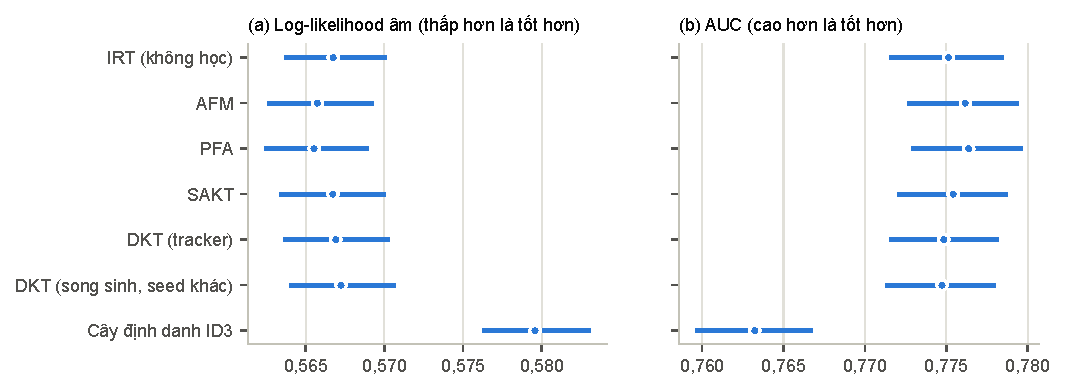
\includegraphics[width=\linewidth]{figures/fig_forecast.pdf}
\caption{Độ chính xác dự báo trên người học giữ lại. (a) Log-likelihood âm và (b) AUC của dự báo lần nộp đầu cho 926 người học kiểm tra (112.950 dự báo); thanh ngang là khoảng tin cậy 95\% bootstrap theo người học. Sáu mô hình thống kê chồng lên nhau; cây định danh dễ diễn giải kém chính xác hơn một chút.}
\label{fig:forecast}
\end{figure}

\subsection{Chính sách trông rất mạnh trong chính bộ mô phỏng huấn luyện}\label{sec:res-insim}

Trong bộ mô phỏng huấn luyện DKT-A, các tác tử thưởng KT cho tiến bộ lớn nhất: PPO nâng post-test kỳ vọng $+$28{,}58 điểm \% và DQN $+$14{,}59 điểm \% sau mười bài, so với $+$1{,}42 điểm \% của chọn ngẫu nhiên; bộ tối đa hóa tham lam một bước theo tracker đạt $+$15{,}31 điểm \% (\cref{tab:matrix}). Các tác tử huấn luyện trong thế giới AFM hoặc nhiều thế giới cũng đạt điểm cao trong DKT-A (ví dụ $+$13{,}11 điểm \% với DQN nhiều thế giới). Nếu đọc riêng lẻ, như thường thấy trong các đánh giá bằng bộ mô phỏng KT, các con số này gợi ý lợi ích lớn của học tăng cường. Tuy nhiên chúng gần như hoàn toàn là độ trôi: trong DKT-A, nơi kết quả do chính tracker sinh ra, phần bất ngờ trong \eqref{eq:decomposition} có trung bình từ $-$0{,}70 đến 0{,}00 điểm \% trên 14 chính sách (cách 0 tối đa 2{,}3 sai số chuẩn Monte Carlo; các luồng kết quả ngẫu nhiên được dùng chung giữa các chính sách), trong khi độ trôi tích lũy của PPO là 29{,}0 điểm \%, đúng như \cref{prop:insim} dự đoán (kiểm tra thăm dò).

\begin{table*}[t]
\centering
\caption{Tiến bộ post-test do thế giới đo (điểm \% sau mười bài) của mọi chính sách trong mọi thế giới đánh giá.}
\label{tab:matrix}
\footnotesize
\resizebox{\textwidth}{!}{%
\begin{tabular}{lrrrrrrrrr}
\toprule
Chính sách & DKT-A$^\dagger$ & AFM-A$^\dagger$ & DKT-A song sinh & DKT-B & SAKT-B & AFM-B & PFA-B & ZPD-B & IRT-B \\
\midrule
Ngẫu nhiên & 1{,}42 & 1{,}83 & 3{,}33 & 1{,}31 & 3{,}36 & 1{,}72 & 1{,}63 & 1{,}93 & 0{,}00 \\
Lộ trình dễ $\to$ khó & 3{,}51 & 0{,}54 & $-$2{,}12 & 2{,}34 & 14{,}17 & 0{,}53 & 0{,}63 & 0{,}52 & 0{,}00 \\
Kỹ năng yếu nhất & 4{,}92 & 1{,}30 & 1{,}93 & 5{,}15 & 3{,}48 & 0{,}97 & 0{,}95 & 0{,}92 & 0{,}00 \\
Nhắm P(đúng) = 0{,}5 & $-$0{,}86 & 1{,}75 & 2{,}58 & $-$0{,}97 & 2{,}32 & 1{,}66 & 1{,}51 & 2{,}18 & 0{,}00 \\
Nhắm P(đúng) = 0{,}7 & 4{,}04 & 1{,}88 & 4{,}45 & $-$1{,}23 & 6{,}88 & 1{,}92 & 2{,}03 & 2{,}13 & 0{,}00 \\
Dễ nhất trước & 0{,}60 & 0{,}91 & 8{,}15 & 5{,}12 & 8{,}31 & 0{,}86 & 0{,}84 & 0{,}70 & 0{,}00 \\
Khó nhất trước & 3{,}31 & 2{,}62 & 7{,}30 & 2{,}16 & 0{,}49 & 2{,}72 & 2{,}19 & 1{,}37 & 0{,}00 \\
Tham lam theo tracker & 15{,}31 & 2{,}02 & 9{,}00 & $-$2{,}99 & 5{,}70 & 2{,}35 & 2{,}42 & 2{,}00 & 0{,}00 \\
DQN (thưởng DKT) & 14{,}59 & 1{,}72 & 10{,}46 & 7{,}57 & 4{,}10 & 1{,}84 & 1{,}82 & 1{,}68 & 0{,}00 \\
PPO (thưởng DKT) & 28{,}58 & 1{,}65 & 13{,}40 & 2{,}71 & 9{,}24 & 2{,}04 & 1{,}97 & 1{,}88 & 0{,}00 \\
DQN (thế giới AFM) & 5{,}06 & 3{,}07 & 4{,}48 & 0{,}46 & 5{,}27 & 3{,}24 & 3{,}35 & 2{,}59 & 0{,}00 \\
PPO (thế giới AFM) & 7{,}15 & 3{,}05 & 7{,}95 & 0{,}00 & 2{,}83 & 3{,}14 & 3{,}34 & 2{,}30 & 0{,}00 \\
DQN (nhiều thế giới) & 13{,}11 & 1{,}92 & 7{,}22 & 1{,}63 & 7{,}52 & 2{,}11 & 1{,}94 & 2{,}09 & 0{,}00 \\
PPO (nhiều thế giới) & 11{,}54 & 2{,}76 & 5{,}89 & 1{,}98 & 5{,}72 & 3{,}07 & 3{,}08 & 2{,}25 & 0{,}00 \\
Oracle một bước & -- & 3{,}20 & -- & -- & -- & 3{,}48 & 3{,}97 & 3{,}64 & 0{,}00 \\
\bottomrule
\end{tabular}}
\par\smallskip
\begin{minipage}{\textwidth}\footnotesize
\textit{Ghi chú.} Trung bình trên 926 lượt đánh giá và, với tác tử học, trên ba seed huấn luyện. $^\dagger$Thế giới huấn luyện. Thế giới DKT và SAKT được đo bằng dự báo của chính chúng; thế giới AFM, PFA và ZPD bằng trạng thái ẩn; IRT-B không có học nên mọi tiến bộ thật bằng 0. Khoảng tin cậy 95\% có trong tệp bổ sung \texttt{evaluation\_matrix\_long.csv}.
\end{minipage}
\end{table*}

\subsection{H1: lợi thế trong mô phỏng không đứng vững ở các thế giới độc lập}\label{sec:res-h1}

So với chọn ngẫu nhiên, DQN với phần thưởng DKT hơn $+$13{,}17 điểm \% [12{,}56; 13{,}73] trong DKT-A, nhưng chỉ $+$7{,}12 điểm \% ở bản song sinh, $+$6{,}26 điểm \% ở DKT-B, $+$0{,}74 điểm \% ở SAKT-B, và $+$0{,}12, $+$0{,}19 và $-$0{,}25 điểm \% ở các thế giới ẩn AFM-B, PFA-B và ZPD-B. Với PPO, lợi thế trong mô phỏng là $+$27{,}16 điểm \% [26{,}54; 27{,}74], so với $+$10{,}07, $+$1{,}40, $+$5{,}87, $+$0{,}32, $+$0{,}34 và $-$0{,}05 điểm \% ở cùng sáu thế giới. Mọi hiệu (trong mô phỏng trừ thế giới độc lập) đều dương với khoảng tin cậy không chứa 0 (nhỏ nhất: DQN so với bản song sinh, $+$6{,}04 điểm \% [5{,}27; 6{,}80]), ủng hộ H1. Trong một so sánh thăm dò, thứ hạng chính sách trong DKT-A chỉ liên hệ yếu với thứ hạng ở các thế giới khác (Kendall $\tau$ = 0{,}49 với bản song sinh, 0{,}05 với DKT-B, 0{,}23 với SAKT-B, 0{,}27 với AFM-B, 0{,}27 với PFA-B và 0{,}08 với ZPD-B). Các thế giới nơ-ron cũng bất đồng với nhau: lộ trình dễ$\to$khó tiến bộ 14{,}17 điểm \% trong SAKT-B nhưng $-$2{,}12 điểm \% trong bản song sinh DKT, nơi chọn ngẫu nhiên đạt 3{,}33 điểm \% (\cref{fig:matrix}).

\begin{figure}[t]
\centering
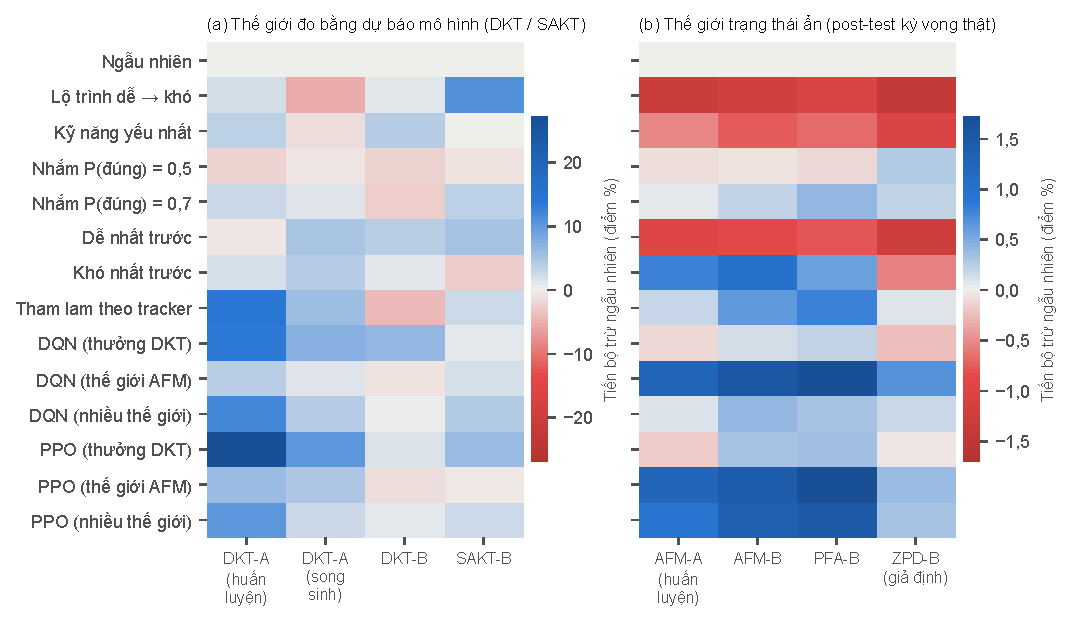
\includegraphics[width=\linewidth]{figures/fig_evaluation_matrix.pdf}
\caption{Tiến bộ so với chọn ngẫu nhiên trong từng thế giới. (a) Các thế giới đo bằng dự báo của chính một mô hình KT nơ-ron; (b) các thế giới có trạng thái ẩn đã biết. Ô xanh: tiến bộ post-test mô phỏng nhiều hơn ngẫu nhiên; ô đỏ: ít hơn. Thang màu của hai panel khác nhau; giá trị và khoảng tin cậy 95\% có trong tệp bổ sung \texttt{evaluation\_matrix\_long.csv}.}
\label{fig:matrix}
\end{figure}

\subsection{H2 và H3: tiến bộ lớn được báo cáo ở nơi không thể có học}\label{sec:res-h2}

Trong thế giới đối chứng âm IRT-B, tiến bộ post-test thật của mọi chính sách đúng bằng 0 theo cách xây dựng. Dù vậy, tracker DKT triển khai vẫn báo tiến bộ $+$12{,}57 điểm \% [11{,}97; 13{,}19] cho bộ tối đa hóa tham lam, $+$12{,}79 điểm \% [12{,}17; 13{,}42] cho DQN và $+$25{,}72 điểm \% [25{,}06; 26{,}38] cho PPO, ủng hộ H2 (\cref{fig:phantom}). Tiến bộ được báo cáo phụ thuộc mạnh vào chính sách: $+$1{,}76 điểm \% với chọn ngẫu nhiên và $+$5{,}56 điểm \% với DQN huấn luyện trong thế giới AFM. Trên 14 chính sách không phải oracle, tiến bộ trong bộ mô phỏng huấn luyện và tiến bộ ảo trong thế giới không học tương quan thứ hạng gần như hoàn hảo (Spearman $\rho$ = 0{,}960), ủng hộ H3 (\cref{fig:insim}): thứ hạng mà đánh giá trong mô phỏng tiêu chuẩn tạo ra về cơ bản là thứ hạng của mức học mà tracker gán cho các lựa chọn bài của chính sách khi thực tế không có học. Các mô hình khác fit trên A ít bị ảnh hưởng hơn nhiều (thăm dò; \cref{tab:observers}): trong IRT-B, AFM và PFA báo tiến bộ tối đa 2{,}91 và 2{,}26 điểm \% với bất kỳ chính sách nào trong số này, còn mô hình IRT tĩnh báo từ $-$0{,}29 đến 0{,}07 điểm \%, tức gần như không có.

\begin{figure}[t]
\centering
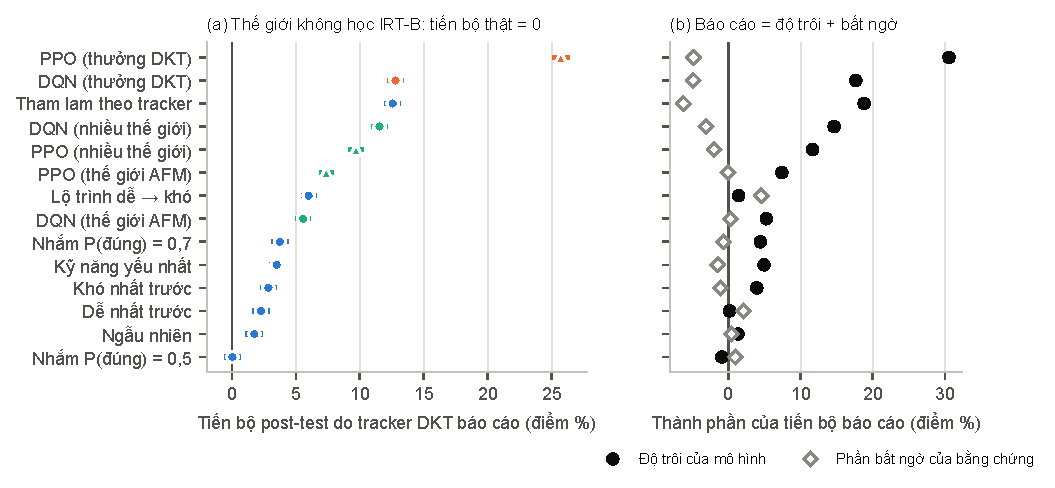
\includegraphics[width=\linewidth]{figures/fig_phantom_gain.pdf}
\caption{Đối chứng âm. (a) Tiến bộ post-test do tracker DKT báo cáo trong thế giới không học IRT-B, nơi tiến bộ thật của mọi chính sách bằng 0 (khoảng tin cậy 95\%). (b) Phân rã chính xác tiến bộ báo cáo thành độ trôi của tracker và phần bất ngờ của bằng chứng (phương trình \eqref{eq:decomposition}).}
\label{fig:phantom}
\end{figure}

\begin{figure}[t]
\centering
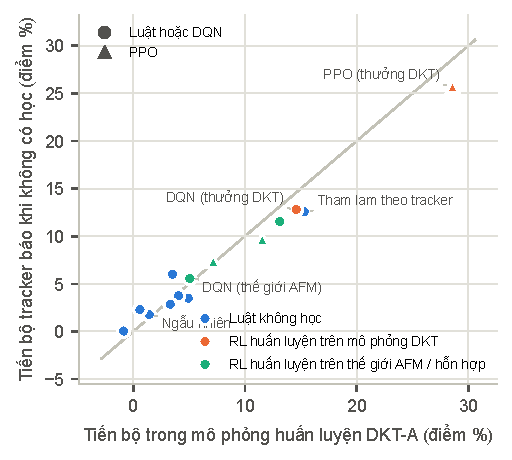
\includegraphics[width=0.62\linewidth]{figures/fig_in_sim_vs_phantom.pdf}
\caption{Tiến bộ trong mô phỏng DKT-A so với tiến bộ ảo mà tracker báo cáo trong thế giới không học IRT-B cho 14 chính sách (Spearman $\rho$ = 0{,}960). Đường chéo xám là $y=x$; hình tam giác là các tác tử PPO.}
\label{fig:insim}
\end{figure}

\subsection{H4: tiến bộ ảo đến từ đâu}\label{sec:res-h4}

Phép phân rã \eqref{eq:decomposition} quy tiến bộ ảo cho độ trôi: trong IRT-B, thay đổi dự báo mà tracker tự kỳ vọng cộng lại bằng $+$30{,}55 điểm \% với PPO, $+$17{,}65 điểm \% với DQN và $+$18{,}79 điểm \% với bộ tối đa hóa tham lam, bị bù trừ một phần bởi phần bất ngờ âm vì thế giới kém thuận lợi hơn tracker kỳ vọng. Mức học ngầm định của một lần luyện phân tán mạnh hơn nhiều ở các mô hình nơ-ron so với các mô hình có số hạng học tường minh (\cref{fig:implied}): độ lệch chuẩn của độ trôi theo bài là 3{,}31 điểm \% với DKT, 3{,}15 với bản song sinh và 2{,}01 với SAKT, so với 0{,}20 với AFM, 0{,}16 với PFA và đúng 0{,}00 với IRT, như \cref{prop:nodrift} đòi hỏi. Hiệu DKT--AFM là 3{,}11 điểm \% [3{,}06; 3{,}16], ủng hộ H4. Trong các phân tích thăm dò, hai DKT — vốn dự báo tốt ngang nhau — chỉ đồng ý yếu về việc bài nào ``dạy'' được (Spearman $\rho$ = 0{,}35 [0{,}34; 0{,}36]), và độ trôi của DKT cao hơn ở các bài được làm nhiều ($\rho$ = 0{,}32) và các bài dễ hơn ($\rho$ = $-$0{,}26 với độ khó IRT) nhưng không liên quan tới vị trí điển hình trong môn học ($\rho$ = $-$0{,}09).

Dọc theo mười tương tác thật tiếp theo của chính người học (905 người học; thăm dò), dự báo post-test của tracker trung bình chỉ dịch chuyển $+$0{,}41 điểm \%, dù trị tuyệt đối của dịch chuyển trung bình là 9{,}43 điểm \%, so với 2{,}42 điểm \% của IRT. Như vậy trên các chuỗi mà người học thật sự đi qua, độ trôi của DKT phần lớn tự triệt tiêu; chỉ khi một chính sách chọn bài vì độ trôi của chúng thì độ trôi mới cộng dồn thành tiến bộ hai chữ số.

\begin{figure}[t]
\centering
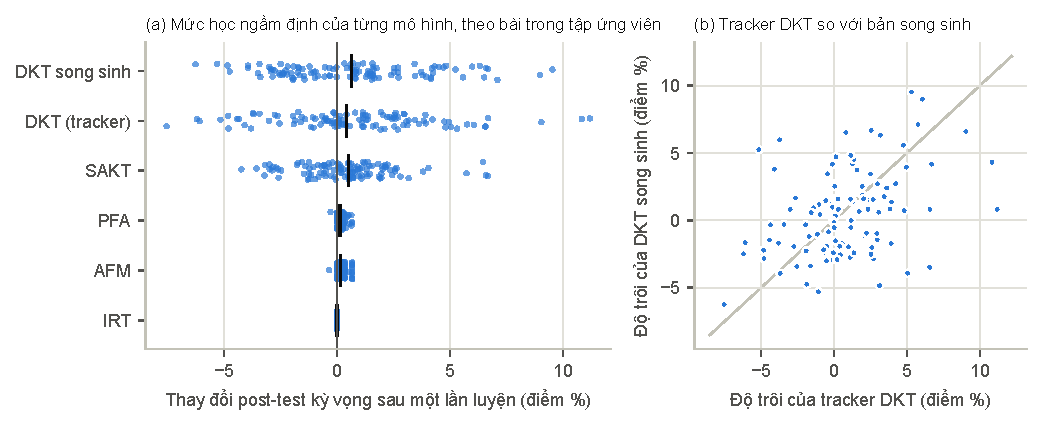
\includegraphics[width=\linewidth]{figures/fig_implied_learning.pdf}
\caption{Mức học ngầm định của từng mô hình. (a) Thay đổi post-test kỳ vọng sau một lần luyện mỗi bài trong tập ứng viên (độ trôi), trung bình trên 300 trạng thái xuất phát; vạch dọc là trung vị. (b) Độ trôi của tracker DKT so với bản song sinh huấn luyện lại (Spearman $\rho$ = 0{,}35); đường chéo xám là $y=x$.}
\label{fig:implied}
\end{figure}

\subsection{Thăm dò: chính sách nào chuyển giao được}\label{sec:res-latent}

Trong các thế giới trạng thái ẩn, khoảng cách giữa các chính sách nhỏ nhưng nhất quán (\cref{fig:effort}). Tác tử huấn luyện trong thế giới AFM là các chính sách không đặc quyền tốt nhất: trong AFM-B, DQN huấn luyện với AFM đạt 3{,}24 điểm \% và PPO 3{,}14 điểm \%, so với 1{,}72 điểm \% của chọn ngẫu nhiên và 3{,}48 điểm \% của oracle một bước có đặc quyền; trong PFA-B, các giá trị tương ứng là 3{,}35, 3{,}34, 1{,}63 và 3{,}97 điểm \%. Trong thế giới độ khó mong muốn giả định ZPD-B, khoảng cách nhỏ hơn (2{,}59 và 2{,}30 so với 1{,}93 điểm \%). Lợi thế so với ngẫu nhiên trong trường hợp xấu nhất trên ba thế giới ẩn là $+$0{,}66 điểm \% với DQN và $+$0{,}37 điểm \% với PPO, lớn nhất trong mọi chính sách, trong khi các tác tử thưởng KT có trường hợp xấu nhất $-$0{,}25 và $-$0{,}05 điểm \%; PPO huấn luyện trên nhiều thế giới đạt gần như vậy ($+$0{,}32 điểm \%). Tác tử huấn luyện với AFM cũng cần ít lượt nộp thêm hơn (6{,}4 và 5{,}0 lượt trên mười bài trong AFM-B, so với 10{,}8 của chọn ngẫu nhiên).

Độ bền này có giới hạn rõ ràng. AFM-B, PFA-B và ZPD-B có chung cấu trúc logistic cộng với thế giới huấn luyện AFM, nên việc chuyển giao giữa chúng một phần là do cách xây dựng. Trong các thế giới nơ-ron, vốn không chia sẻ cấu trúc đó, lợi thế so với ngẫu nhiên của các tác tử huấn luyện với AFM dao động từ $-$1{,}31 đến $+$4{,}62 điểm \% và âm trong DKT-B ($-$0{,}86 và $-$1{,}31 điểm \%). Các luật nhắm xác suất đúng dự báo 0,7 nhỉnh hơn ngẫu nhiên ở mọi thế giới ẩn (trường hợp xấu nhất $+$0{,}20 điểm \%), trong khi lộ trình dễ$\to$khó và luật chọn bài dễ nhất trước luôn kém nhất trong các thế giới ẩn, vì dành lượt luyện cho những bài người học vốn đã giải được.

\begin{figure}[t]
\centering
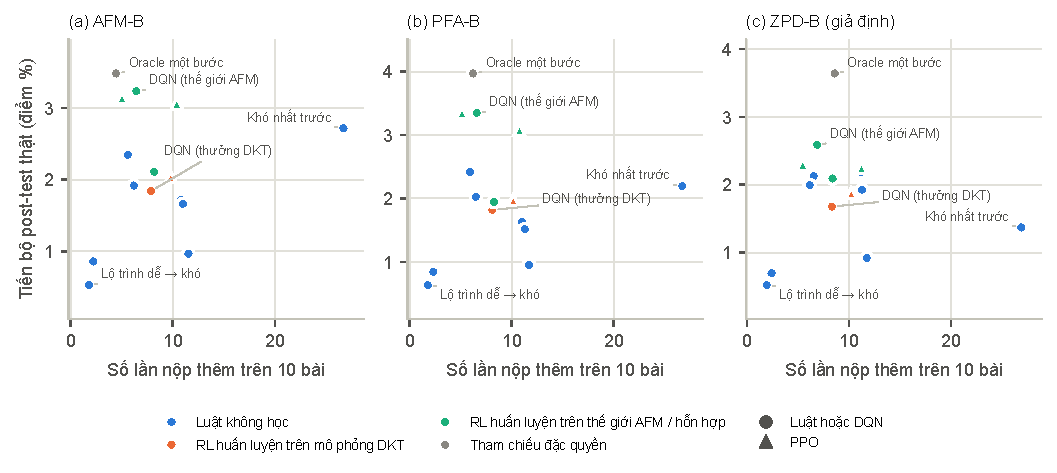
\includegraphics[width=\linewidth]{figures/fig_gain_effort.pdf}
\caption{Tiến bộ post-test thật so với số lượt nộp thêm trên mười bài trong ba thế giới ẩn fit hoặc xây dựng từ phân vùng B: (a) AFM-B, (b) PFA-B và (c) thế giới độ khó mong muốn giả định ZPD-B. Màu phân biệt các họ chính sách, hình tam giác đánh dấu tác tử PPO.}
\label{fig:effort}
\end{figure}

\section{Thảo luận}\label{sec:discussion}

\subsection{Tiến bộ trong mô phỏng thực chất đo cái gì}

Phát hiện trung tâm là: trên dữ liệu lập trình thật, tiến bộ của một chính sách bên trong bộ mô phỏng KT chủ yếu đo mức học mà mô hình của bộ mô phỏng \emph{tin rằng} các lựa chọn bài của nó tạo ra, chứ không phải mức người học sẽ học được. \Cref{prop:insim} phát biểu điều này chính xác: khi một mô hình KT vừa là bộ mô phỏng vừa là thước đo, tiến bộ báo cáo kỳ vọng của mọi chính sách là độ trôi tích lũy của nó, và phần bất ngờ đo được trong DKT-A quả thực không đáng kể. Sáu mô hình người học có độ chính xác dự báo tương đương lại hàm ý mức học rất khác nhau: các mô hình có học tường minh gán cho việc luyện tập những tiến bộ nhỏ và đồng đều, trong khi hai DKT gán tiến bộ vài điểm phần trăm cho từng bài riêng lẻ, theo những hướng mà một seed ngẫu nhiên thứ hai chỉ tái lập yếu. Đây là một trường hợp của tính thiếu xác định (underspecification) \citep{damour2022underspecification}: dữ liệu ràng buộc dự báo bước kế tiếp — điều mọi mô hình đều khớp — nhưng không ràng buộc hệ quả phản thực tế của những chuỗi luyện tập mà người học chưa từng đi qua. Kết quả này mở rộng nhận xét rằng các mô hình người học có độ chính xác tương tự có thể kê đơn lượng luyện tập khác nhau \citep{lee2012individualizing,rollinson2015predictive} từ quyết định về mức thành thạo sang các chính sách sắp xếp trình tự được tối ưu, nơi sự bất đồng bị khuếch đại chứ không chỉ lộ ra. Học tăng cường là một cách tìm kiếm hiệu quả chính những chuỗi như vậy. Bộ tối ưu mạnh hơn (PPO) khai thác phần thưởng DKT nhiều nhất, đạt tiến bộ trong mô phỏng khoảng gấp đôi DQN và một tiến bộ ảo có cùng độ lớn trong thế giới không học.

Hai quan sát nữa làm rõ cách diễn giải. Thứ nhất, với một chính sách cho trước, tiến bộ mà tracker báo cáo thay đổi rất ít giữa chín thế giới — với PPO thưởng DKT trong khoảng 25{,}7 đến 28{,}6 điểm \%, với chọn ngẫu nhiên từ 0{,}6 đến 2{,}6 điểm \%: giá trị của nó chủ yếu do chính sách chọn bài nào quyết định, chứ không do người học mô phỏng phản ứng ra sao. Thứ hai, dọc theo chuỗi tiếp diễn thật của người học, độ trôi của DKT tự triệt tiêu; dự báo của nó dao động mạnh, như đã được ghi nhận với DKT \citep{yeung2018dktplus}, nhưng không lệch có hệ thống ở đó. Vấn đề phát sinh ngoài phân phối dữ liệu, nơi chính sách cộng dồn độ trôi bước này sang bước khác. Kiểm định dự báo trên chuỗi đã ghi log không thể phát hiện kiểu thất bại này; đó là lý do các mô hình không phân biệt được trong \cref{tab:forecast} vẫn có thể bất đồng về chính sách.

\subsection{Liên hệ với khai thác sai số mô hình và tối ưu quá mức phần thưởng}

Tiến bộ ảo là phiên bản giáo dục của hiện tượng khai thác sai số mô hình trong RL dựa trên mô hình và của việc tối ưu quá mức phần thưởng: một tác tử được tối ưu trên mô hình học từ dữ liệu sẽ tìm ra những hành động mà mô hình lạc quan nhất \citep{kurutach2018metrpo,janner2019trust,gao2023scaling,skalse2022reward}. Bộ gợi ý KT--RL đặc biệt dễ tổn thương vì cùng một mô hình học từ dữ liệu cung cấp động học, phần thưởng và phép đánh giá, nên đánh giá bên trong mô hình đó không thể lộ ra sự khai thác. Các biện pháp phát triển trong RL dựa trên mô hình gợi ý những thiết kế có thể kiểm định cho bộ gợi ý giáo dục: phạt mức bất đồng của một tổ hợp tracker, mà bản song sinh của chúng tôi là trường hợp tối thiểu \citep{kurutach2018metrpo,yu2020mopo}; giới hạn lập kế hoạch ở chân trời ngắn hoặc ở các bài có nhiều dữ liệu \citep{janner2019trust}; hoặc ràng buộc mô hình người học để độ trôi diễn giải được và đơn điệu \citep{zhang2023cmkt}. Chúng tôi chưa đánh giá các biện pháp này, và liệu chúng có khôi phục được tiến bộ học thật hay không vẫn là câu hỏi mở.

\subsection{Hàm ý cho việc đánh giá hệ gợi ý thích ứng}

Kết quả của chúng tôi không cho thấy các hệ thống đã công bố mà chúng tôi dựa vào là sai; chúng tôi không tái lập nhiệm vụ, phần thưởng hay dữ liệu của họ. Kết quả cho thấy một thiết kế chung của nhiều hệ thống — huấn luyện và chấm điểm chính sách bằng cùng một mô hình KT đã fit, hoặc bằng các mô hình fit trên cùng log — có thể báo cáo cải thiện lớn cho những chính sách không dạy được gì. Vì vậy chúng tôi đề xuất bốn kiểm tra ít tốn kém cho các nghiên cứu gợi ý bài tập dựa trên mô phỏng. (i) Báo cáo \emph{đối chứng âm}: đánh giá mọi chính sách trong một thế giới không có học, nơi tiến bộ thật được biết là bằng 0, và báo cáo tiến bộ mà tracker tuyên bố ở đó. (ii) Báo cáo \emph{phép phân rã độ trôi} ở phương trình \eqref{eq:decomposition}, chỉ cần tracker và phơi bày những tiến bộ mà mô hình tự kỳ vọng. (iii) Đánh giá trong các \emph{thế giới fit độc lập} với cấu trúc học và người học khác nhau, theo ma trận đánh giá bền vững \citep{doroudi2017rem}, gồm ít nhất một thế giới có tham số học tường minh. (iv) Fit lại tracker với seed khác và báo cáo mức đồng thuận về mức học ngầm định. Không kiểm tra nào trong số này cần dữ liệu học sinh ngoài log đã dùng. Vì kết quả RL thay đổi theo seed huấn luyện, các kiểm tra nên được báo cáo theo từng seed hoặc kèm độ bất định ở mức seed \citep{henderson2018matters,agarwal2021precipice}.

\subsection{Học tăng cường có thể đóng góp gì}

Học tăng cường không vô dụng. Khi thế giới huấn luyện có cấu trúc học tường minh, diễn giải được (AFM), DQN và PPO học được các chính sách chuyển giao sang các thế giới AFM và PFA fit độc lập và sang một thế giới có quy luật học giả định khác, tiệm cận oracle một bước có đặc quyền trong khi tốn ít lượt nộp hơn chọn ngẫu nhiên. Điều này phù hợp với nhận xét của \citet{doroudi2019reward} rằng chính sách rút ra từ mô hình có ràng buộc lý thuyết đáng tin hơn chính sách rút ra từ mô hình thuần dữ liệu không ràng buộc. Tuy vậy bằng chứng còn hạn chế: tiến bộ khiêm tốn — từ 1{,}4 đến 1{,}7 điểm \% xác suất đúng post-test kỳ vọng so với chọn ngẫu nhiên sau mười bài trong AFM-B và PFA-B — vẫn là đại lượng mô phỏng, các thế giới ẩn có chung cấu trúc với thế giới AFM, và chính các tác tử này không vượt chọn ngẫu nhiên trong DKT-B. Các luật nhắm xác suất đúng dự báo vừa phải (0,7) cũng bền vững, trong khi lộ trình dễ$\to$khó và chọn bài dễ nhất trước — thái cực ``quá dễ'' trong lập luận vùng phát triển gần của đề tài — luôn kém hiệu quả nhất trong các thế giới ẩn.

\subsection{Giới hạn}

Mọi kết quả về chính sách đều là mô phỏng. Các thế giới ẩn được fit trên log quan sát của một nền tảng và một nhóm môn học; hệ số học của chúng là các liên hệ đã điều chỉnh theo năng lực và độ khó của bài, không phải hiệu ứng nhân quả, và thế giới ZPD là một giả định. Vì các thế giới ẩn có chung cấu trúc logistic cộng, độ bền của các tác tử huấn luyện với AFM là có điều kiện trên cấu trúc đó. Cách gom kỹ năng là của chúng tôi, và con trỏ — dù nổi bật trong mô tả đề tài — chỉ có một bài trong tập ứng viên vì ít bài con trỏ đạt ngưỡng hỗ trợ 5\%. Công sức được đo bằng số lượt nộp, không phải thời gian làm bài. Chúng tôi nghiên cứu kết quả lần nộp đầu, chân trời mười bài và một trọng số công sức duy nhất; chân trời dài hơn, phần thưởng khác và tập ứng viên khác có thể thay đổi độ lớn kết quả, và chúng tôi chưa phân tích độ nhạy cho các lựa chọn này. Mỗi tác tử được huấn luyện với ba seed, và khoảng tin cậy có điều kiện trên các seed này và trên các mô hình đã fit; chúng không được hiệu chỉnh cho so sánh bội, dù mọi phép so sánh đăng ký trước đều được báo cáo, và các tương quan thứ hạng được tính trên những chính sách không độc lập với nhau. Dữ liệu đến từ hệ thống chấm bài của một trường đại học, nên khả năng khái quát sang ngôn ngữ lập trình, thiết kế môn học và quần thể người học khác chưa được kiểm chứng. Cuối cùng, chúng tôi không thử bất kỳ chính sách nào với học sinh; bằng chứng liên quan tới tính hợp lệ của đánh giá dựa trên mô phỏng và độ bền tương đối của các chính sách trên các thế giới hợp lý, chứ không phải tiến bộ học tập của người học thật.

\section{Kết luận}\label{sec:conclusion}

Chúng tôi đã xây dựng và đánh giá một bộ gợi ý bài tập thích ứng cho lập trình C hoàn toàn từ log người học thật: các mô hình người học gồm DKT và một cây định danh dựa trên entropy, một bài toán quyết định tuần tự có phần thưởng kết hợp tiến bộ post-test và công sức giải bài, cùng các tác tử DQN và PPO. Các mô hình người học dự báo tốt ngang nhau, nhưng tác tử huấn luyện trên bộ mô phỏng DKT đạt những tiến bộ lớn không đứng vững trong các thế giới fit độc lập, và tracker cũng báo những tiến bộ đó khi việc học là không thể. Chúng tôi chứng minh rằng tiến bộ trong mô phỏng như vậy, xét theo kỳ vọng, chính là độ trôi tích lũy của tracker — mức học mà mô hình tự hứa với chính nó — điều mà một mô hình nhất quán không có học không bao giờ báo cáo, và một DKT huấn luyện lại với seed khác không tái lập được. Tác tử huấn luyện với mô hình học tường minh chuyển giao tốt nhất trong họ các thế giới ẩn, nhưng không sang các thế giới nơ-ron. Với các nhà nghiên cứu và nhà phát triển hệ gợi ý thích ứng, thông điệp thực tiễn là: kèm mọi đánh giá dựa trên mô phỏng bằng một thế giới đối chứng âm, phép phân rã độ trôi và các thế giới fit độc lập, và dè dặt với tiến bộ trong mô phỏng của các chính sách đã được tối ưu cho tới khi chúng vượt qua các kiểm tra này. Cần lặp lại trên các bộ dữ liệu khác, phân tích độ nhạy của bài toán quyết định và cuối cùng là một nghiên cứu có đối chứng với học sinh để xác định các chính sách bền vững có thực sự giúp người học thật hay không; pipeline và ứng dụng của chúng tôi được thiết kế để hỗ trợ các nghiên cứu đó.

\appendix
\section{Chứng minh}\label{app:proofs}

\paragraph{Chứng minh \cref{prop:nodrift}} Đặt $\bar p(\theta)=|\mathcal W|^{-1}\sum_{k\in\mathcal W}p(y=1\mid k,\theta)$ và gọi $\pi_H$ là phân phối hậu nghiệm của $\theta$ sau lịch sử $H$. Dự báo của mô hình là dự báo hậu nghiệm, $\bar P_M(H)=\int\bar p(\theta)\,\pi_H(\mathrm d\theta)$ và $P_M(y\mid j,H)=\int p(y\mid j,\theta)\,\pi_H(\mathrm d\theta)$. Vì $\theta$ không đổi theo luyện tập và các kết quả độc lập có điều kiện khi biết $\theta$, quy tắc Bayes cho $\pi_{H\oplus(j,y)}(\mathrm d\theta)=p(y\mid j,\theta)\,\pi_H(\mathrm d\theta)/P_M(y\mid j,H)$. Do đó
\begin{align}
\sum_{y\in\{0,1\}}P_M(y\mid j,H)\,\bar P_M\bigl(H\oplus(j,y)\bigr)
&=\sum_{y\in\{0,1\}}\int\bar p(\theta)\,p(y\mid j,\theta)\,\pi_H(\mathrm d\theta)\notag\\
&=\int\bar p(\theta)\,\pi_H(\mathrm d\theta)=\bar P_M(H),
\end{align}
tức là $D_M(j,H)=0$. Lập luận đúng với mọi phân phối tiên nghiệm, kể cả lưới hữu hạn dùng cho IRT trong nghiên cứu này; độ trôi theo từng bài của IRT đúng bằng 0 (\cref{sec:res-h4}). $\square$

\paragraph{Chứng minh \cref{prop:insim}} Gọi $S_t=\bar P_M(H_{t+1})-\bar P_M(H_t)-D_M(j_t,H_t)$ là phần bất ngờ ở bước $t$. Nếu $y_t$ được rút từ $P_M(\cdot\mid j_t,H_t)$ thì theo \eqref{eq:drift}
\begin{align}
\mathbb E\bigl[S_t\mid H_t,j_t\bigr]
&=\sum_{y\in\{0,1\}}P_M(y\mid j_t,H_t)\,\bar P_M\bigl(H_t\oplus(j_t,y)\bigr)\notag\\
&\quad-\bar P_M(H_t)-D_M(j_t,H_t)=0.
\end{align}
Lựa chọn $j_t$ chỉ phụ thuộc $H_t$ và vào yếu tố ngẫu nhiên độc lập với các kết quả tương lai, nên theo tính chất kỳ vọng lặp $\mathbb E[S_t]=0$ với mọi $t$. Lấy kỳ vọng hai vế của \eqref{eq:decomposition} ta được kết quả. Kết hợp hai mệnh đề: một bộ mô phỏng nhất quán không có học gán tiến bộ kỳ vọng bằng 0 cho mọi chính sách, còn một bộ mô phỏng có học xếp hạng chính sách theo độ trôi mà chúng tích lũy. $\square$

\section{Chi tiết cài đặt}\label{app:impl}

\paragraph{Mô hình người học} Mô hình logistic: tiên nghiệm $\theta\sim\mathcal N(0,\sigma_\theta^2)$ với $\sigma_\theta\in\{0{,}4;\,0{,}5;\,0{,}6;\,0{,}75\}$ chọn theo NLL trên tập kiểm định trong, tham số riêng của bài $\mathcal N(0,1)$, hệ số học $\mathcal N(0,1)$; tối ưu L-BFGS toàn batch. DKT: embedding 32, LSTM 64, dropout 0,3 (0,1 ở đầu vào), AdamW với weight decay $10^{-4}$, tốc độ học $10^{-3}$, batch 32, dừng sớm với độ kiên nhẫn 3 (tối đa 30 epoch). SAKT: chiều 64, 4 đầu chú ý, cửa sổ 200, dropout 0,1. Bài có ít nhất 10 người học trong tập fit có tham số riêng. ID3: lá tối thiểu 200 mẫu, lợi ích thông tin tối thiểu $10^{-3}$, độ sâu tối đa 6.

\paragraph{Tác tử} Trạng thái: 109 xác suất đúng dự báo, 109 cờ hợp lệ, 10 trung bình theo kỹ năng, dự báo post-test và số bước còn lại. Double DQN: hai lớp ẩn 256, bộ nhớ replay 50.000, batch 256, tốc độ học $5\times10^{-4}$, cập nhật mạng đích mềm $\tau=0{,}01$, $\varepsilon$ giảm từ 1 xuống 0,05 trong nửa đầu huấn luyện, $\gamma=0{,}99$. PPO: hai lớp ẩn 256 (tanh), tốc độ học $3\times10^{-4}$, 4 epoch, minibatch 128, clip 0,2, hệ số entropy 0,01, GAE $\lambda=0{,}95$. Mỗi tác tử: 300 vòng lặp, mỗi vòng 64 lượt song song dài mười bước; dùng checkpoint cuối; seed 11, 23 và 37. Công sức: sau một lần nộp đầu thất bại, số lần nộp thêm theo phân phối hình học với trung bình của bài lấy từ phân vùng của thế giới (co về trung bình chung, chặn trên ở 10).

\section{Dự báo theo kỹ năng}\label{app:skills}

\begin{table}[H]
\centering
\caption{AUC theo kỹ năng chính của bài cần dự báo (người học kiểm tra T, mô hình fit trên A).}
\label{tab:skills}
\small
\resizebox{\linewidth}{!}{%
\begin{tabular}{lrrrrrrr}
\toprule
Kỹ năng & $n$ & Tỉ lệ nền & IRT & PFA & DKT & SAKT & ID3 \\
\midrule
Cú pháp cơ bản, nhập xuất, kiểu dữ liệu & 44.513 & 0{,}55 & 0{,}774 & 0{,}775 & 0{,}774 & 0{,}775 & 0{,}763 \\
Rẽ nhánh & 4.171 & 0{,}53 & 0{,}761 & 0{,}763 & 0{,}768 & 0{,}763 & 0{,}751 \\
Vòng lặp & 2.528 & 0{,}48 & 0{,}754 & 0{,}758 & 0{,}761 & 0{,}752 & 0{,}745 \\
Mảng & 2.440 & 0{,}50 & 0{,}789 & 0{,}791 & 0{,}790 & 0{,}788 & 0{,}780 \\
Xâu ký tự & 5.999 & 0{,}53 & 0{,}731 & 0{,}733 & 0{,}729 & 0{,}731 & 0{,}716 \\
Con trỏ và danh sách liên kết & 444 & 0{,}66 & 0{,}701 & 0{,}705 & 0{,}699 & 0{,}691 & 0{,}709 \\
Phép toán bit và hệ cơ số & 9.219 & 0{,}50 & 0{,}764 & 0{,}766 & 0{,}764 & 0{,}766 & 0{,}750 \\
Số học và lý thuyết số & 4.557 & 0{,}52 & 0{,}823 & 0{,}824 & 0{,}817 & 0{,}824 & 0{,}812 \\
Đệ quy, truy hồi và chia để trị & 3.344 & 0{,}57 & 0{,}789 & 0{,}790 & 0{,}784 & 0{,}783 & 0{,}777 \\
Sắp xếp và tìm kiếm & 5.433 & 0{,}44 & 0{,}755 & 0{,}757 & 0{,}749 & 0{,}749 & 0{,}737 \\
\bottomrule
\end{tabular}}
\end{table}

\section{Tiến bộ mà các mô hình khác tuyên bố trong đối chứng âm}\label{app:observers}

\begin{table}[H]
\centering
\caption{Tiến bộ post-test (điểm \%) mà mỗi mô hình fit trên A sẽ báo cáo sau cùng các lượt trong thế giới không học IRT-B (thăm dò). Tiến bộ thật bằng 0.}
\label{tab:observers}
\small
\begin{tabular}{lrrrrr}
\toprule
Chính sách & DKT & SAKT & AFM & PFA & IRT \\
\midrule
Ngẫu nhiên & 1{,}76 & 3{,}69 & 1{,}73 & 1{,}40 & $-$0{,}14 \\
Lộ trình dễ $\to$ khó & 6{,}00 & 11{,}12 & 0{,}64 & 0{,}55 & 0{,}06 \\
Nhắm P(đúng) = 0{,}7 & 3{,}75 & 5{,}28 & 1{,}62 & 1{,}20 & $-$0{,}25 \\
Tham lam theo tracker & 12{,}57 & 5{,}58 & 2{,}05 & 1{,}50 & $-$0{,}08 \\
DQN (thưởng DKT) & 12{,}79 & 3{,}87 & 1{,}21 & 0{,}81 & $-$0{,}27 \\
PPO (thưởng DKT) & 25{,}72 & 5{,}93 & 1{,}57 & 1{,}19 & $-$0{,}04 \\
DQN (thế giới AFM) & 5{,}56 & 3{,}45 & 2{,}91 & 2{,}26 & $-$0{,}13 \\
PPO (thế giới AFM) & 7{,}37 & 3{,}54 & 2{,}56 & 1{,}92 & $-$0{,}28 \\
\bottomrule
\end{tabular}
\end{table}

\section{Khả năng tái lập}\label{app:repro}

Cả hai protocol đã được khóa trước khi nạp quần thể đánh giá; bản ghi khóa liệt kê mã băm SHA-256 của protocol và mã nguồn. Các thí nghiệm chạy qua một harness chỉ-ghi-thêm, chụp lại protocol và mã nguồn, ghi mã băm đầu vào và đầu ra, và từ chối ghi đè một run. Bản ghi run: giai đoạn mô hình người học \texttt{10bf859c0486}\ldots, giai đoạn chính sách \texttt{167b9e90f3f3}\ldots\ (tiền tố SHA-256). Việc phát triển và chọn siêu tham số dùng một cohort đã xem trước, tách rời khỏi quần thể đánh giá. Mọi con số trong bản thảo được chèn tự động từ đầu ra của run.

\section*{Tính sẵn có của dữ liệu}
Bộ dữ liệu ACcoding được các tác giả công bố công khai \citep{sun2026accodingdata,chen2024accoding}. Mã nguồn, protocol đã khóa, bản ghi run, kết quả tổng hợp và các bảng số liệu đứng sau mọi hình sẽ được lưu ở kho công khai khi bài được chấp nhận (bản ẩn danh cung cấp cho phản biện khi được yêu cầu); các tệp dẫn xuất ở mức người học không được phân phối lại.

\section*{Tuyên bố đạo đức}
Đây là phân tích thứ cấp trên một bộ dữ liệu công khai đã ẩn danh. Không thu thập dữ liệu mới và không liên hệ hay phân nhóm bất kỳ người học nào.

\section*{Khai báo sử dụng AI tạo sinh và công nghệ hỗ trợ bởi AI trong quá trình chuẩn bị bản thảo}
Trong quá trình chuẩn bị công trình này, (các) tác giả đã dùng Claude (Anthropic), một trợ lý AI, để viết và chạy mã phân tích, mã vẽ hình, và để soạn thảo, chỉnh sửa văn bản. Sau khi dùng công cụ này, (các) tác giả đã rà soát, chỉnh sửa nội dung khi cần và chịu hoàn toàn trách nhiệm về nội dung bài báo. \emph{[Tác giả: xác nhận hoặc sửa tuyên bố này cho đúng thực tế sử dụng trước khi nộp.]}

\begin{thebibliography}{73}
\expandafter\ifx\csname url\endcsname\relax
  \def\url#1{\texttt{#1}}\fi
\bibitem[{Abdelrahman và cộng sự(2023)Abdelrahman, Wang và Nunes}]{abdelrahman2023survey}
Abdelrahman, G., Wang, Q., \& Nunes, B. (2023). Knowledge tracing: A survey. \textit{ACM Computing Surveys}, \textit{55}(11), 1--37. \url{https://doi.org/10.1145/3569576}

\bibitem[{Agarwal và cộng sự(2021)Agarwal, Schwarzer, Castro, Courville và Bellemare}]{agarwal2021precipice}
Agarwal, R., Schwarzer, M., Castro, P. S., Courville, A., \& Bellemare, M. G. (2021). Deep reinforcement learning at the edge of the statistical precipice. In \textit{Advances in Neural Information Processing Systems} (Vol.~34, pp.~29304--29320). Curran Associates.

\bibitem[{Ai và cộng sự(2019)Ai, Chen, Guo, Zhao, Wang, Fu và Wang}]{ai2019cdkt}
Ai, F., Chen, Y., Guo, Y., Zhao, Y., Wang, Z., Fu, G., \& Wang, G. (2019). Concept-aware deep knowledge tracing and exercise recommendation in an online learning system. In \textit{Proceedings of the 12th International Conference on Educational Data Mining} (pp.~240--245). International Educational Data Mining Society. \url{https://eric.ed.gov/?id=ED599194}

\bibitem[{Amodei và cộng sự(2016)Amodei, Olah, Steinhardt, Christiano, Schulman và Mané}]{amodei2016concrete}
Amodei, D., Olah, C., Steinhardt, J., Christiano, P., Schulman, J., \& Mané, D. (2016). \textit{Concrete problems in AI safety} [Preprint]. arXiv. \url{https://doi.org/10.48550/arXiv.1606.06565}

\bibitem[{Arnold và cộng sự(2016)Arnold, Ercumen, Benjamin-Chung và Colford}]{arnold2016negative}
Arnold, B. F., Ercumen, A., Benjamin-Chung, J., \& Colford, J. M. (2016). Brief report: Negative controls to detect selection bias and measurement bias in epidemiologic studies. \textit{Epidemiology}, \textit{27}(5), 637--641. \url{https://doi.org/10.1097/EDE.0000000000000504}

\bibitem[{Bassen và cộng sự(2020)Bassen, Balaji, Schaarschmidt, Thille, Painter, Zimmaro, Games, Fast và Mitchell}]{bassen2020chi}
Bassen, J., Balaji, B., Schaarschmidt, M., Thille, C., Painter, J., Zimmaro, D., Games, A., Fast, E., \& Mitchell, J. C. (2020). Reinforcement learning for the adaptive scheduling of educational activities. In \textit{Proceedings of the 2020 CHI Conference on Human Factors in Computing Systems} (pp.~1--12). ACM. \url{https://doi.org/10.1145/3313831.3376518}

\bibitem[{Breiman(2001)Breiman}]{breiman2001two}
Breiman, L. (2001). Statistical modeling: The two cultures. \textit{Statistical Science}, \textit{16}(3), 199--231. \url{https://doi.org/10.1214/ss/1009213726}

\bibitem[{Brusilovsky và Millán(2007)Brusilovsky và Millán}]{brusilovsky2007user}
Brusilovsky, P., \& Millán, E. (2007). User models for adaptive hypermedia and adaptive educational systems. In P. Brusilovsky, A. Kobsa, \& W. Nejdl (Eds.), \textit{The adaptive web: Methods and strategies of web personalization} (Lecture Notes in Computer Science, Vol.~4321, pp.~3--53). Springer. \url{https://doi.org/10.1007/978-3-540-72079-9_1}

\bibitem[{Cen và cộng sự(2006)Cen, Koedinger và Junker}]{cen2006lfa}
Cen, H., Koedinger, K. R., \& Junker, B. (2006). Learning factors analysis -- A general method for cognitive model evaluation and improvement. In \textit{Intelligent Tutoring Systems: 8th International Conference, ITS 2006} (Lecture Notes in Computer Science, Vol.~4053, pp.~164--175). Springer. \url{https://doi.org/10.1007/11774303_17}

\bibitem[{Chen và cộng sự(2024)Chen, Huang, Liu, Yu, Meng, Mo, Zhang và Song}]{chen2024accoding}
Chen, K., Huang, F., Liu, Z., Yu, H., Meng, L., Mo, S., Zhang, L., \& Song, Y. (2024). ACcoding: A graph-based dataset for online judge programming. \textit{Scientific Data}, \textit{11}, Article 548. \url{https://doi.org/10.1038/s41597-024-03392-z}

\bibitem[{Chen và cộng sự(2023)Chen, Shen, Xia, Jin, Song, Zhang, Liu, Zhu, Tang, Dong, Xia và Yu}]{chen2023src}
Chen, X., Shen, J., Xia, W., Jin, J., Song, Y., Zhang, W., Liu, W., Zhu, M., Tang, R., Dong, K., Xia, D., \& Yu, Y. (2023). Set-to-sequence ranking-based concept-aware learning path recommendation. \textit{Proceedings of the AAAI Conference on Artificial Intelligence}, \textit{37}(4), 5027--5035. \url{https://doi.org/10.1609/aaai.v37i4.25630}

\bibitem[{Cheng và cộng sự(2026)Cheng, Zhuang, Xie, Wang, Liu, Guan, Fang và Pan}]{cheng2026unier}
Cheng, X., Zhuang, G., Xie, Y., Wang, J., Liu, Y., Guan, Q., Fang, L., \& Pan, S. (2026). \textit{UniER: A unified benchmark for item-level and path-level exercise recommendation} [Preprint]. arXiv. \url{https://doi.org/10.48550/arXiv.2605.16750}

\bibitem[{Chi và cộng sự(2011)Chi, VanLehn, Litman và Jordan}]{chi2011umuai}
Chi, M., VanLehn, K., Litman, D., \& Jordan, P. (2011). Empirically evaluating the application of reinforcement learning to the induction of effective and adaptive pedagogical strategies. \textit{User Modeling and User-Adapted Interaction}, \textit{21}(1--2), 137--180. \url{https://doi.org/10.1007/s11257-010-9093-1}

\bibitem[{Clement và cộng sự(2015)Clement, Roy, Oudeyer và Lopes}]{clement2015bandits}
Clement, B., Roy, D., Oudeyer, P.-Y., \& Lopes, M. (2015). Multi-armed bandits for intelligent tutoring systems. \textit{Journal of Educational Data Mining}, \textit{7}(2), 20--48. \url{https://doi.org/10.5281/zenodo.3554667}

\bibitem[{Corbett và Anderson(1994)Corbett và Anderson}]{corbett1994bkt}
Corbett, A. T., \& Anderson, J. R. (1994). Knowledge tracing: Modeling the acquisition of procedural knowledge. \textit{User Modeling and User-Adapted Interaction}, \textit{4}(4), 253--278. \url{https://doi.org/10.1007/BF01099821}

\bibitem[{D'Amour và cộng sự(2022)D'Amour, Heller, Moldovan, Adlam, Alipanahi, Beutel, Chen, Deaton, Eisenstein, Hoffman, Hormozdiari, Houlsby, Hou, Jerfel, Karthikesalingam, Lucic, Ma, McLean, Mincu, Mitani, Montanari, Nado, Natarajan, Nielson, Osborne, Raman, Ramasamy, Sayres, Schrouff, Seneviratne, Sequeira, Suresh, Veitch, Vladymyrov, Wang, Webster, Yadlowsky, Yun, Zhai và Sculley}]{damour2022underspecification}
D'Amour, A., Heller, K., Moldovan, D., Adlam, B., Alipanahi, B., Beutel, A., Chen, C., Deaton, J., Eisenstein, J., Hoffman, M. D., Hormozdiari, F., Houlsby, N., Hou, S., Jerfel, G., Karthikesalingam, A., Lucic, M., Ma, Y., McLean, C., Mincu, D., \ldots\ Sculley, D. (2022). Underspecification presents challenges for credibility in modern machine learning. \textit{Journal of Machine Learning Research}, \textit{23}(226), 1--61. \url{https://jmlr.org/papers/v23/20-1335.html}

\bibitem[{Doroudi và cộng sự(2017)Doroudi, Aleven và Brunskill}]{doroudi2017rem}
Doroudi, S., Aleven, V., \& Brunskill, E. (2017). Robust evaluation matrix: Towards a more principled offline exploration of instructional policies. In \textit{Proceedings of the Fourth ACM Conference on Learning @ Scale} (pp.~3--12). ACM. \url{https://doi.org/10.1145/3051457.3051463}

\bibitem[{Doroudi và cộng sự(2019)Doroudi, Aleven và Brunskill}]{doroudi2019reward}
Doroudi, S., Aleven, V., \& Brunskill, E. (2019). Where's the reward? A review of reinforcement learning for instructional sequencing. \textit{International Journal of Artificial Intelligence in Education}, \textit{29}(4), 568--620. \url{https://doi.org/10.1007/s40593-019-00187-x}

\bibitem[{Doroudi và Brunskill(2017)Doroudi và Brunskill}]{doroudi2017identifiability}
Doroudi, S., \& Brunskill, E. (2017). The misidentified identifiability problem of Bayesian knowledge tracing. In \textit{Proceedings of the 10th International Conference on Educational Data Mining} (pp.~143--149). International Educational Data Mining Society. \url{https://eric.ed.gov/?id=ED596611}

\bibitem[{Doroudi và Brunskill(2019)Doroudi và Brunskill}]{doroudi2019fairer}
Doroudi, S., \& Brunskill, E. (2019). Fairer but not fair enough: On the equitability of knowledge tracing. In \textit{Proceedings of the 9th International Conference on Learning Analytics \& Knowledge} (pp.~335--339). ACM. \url{https://doi.org/10.1145/3303772.3303838}

\bibitem[{Dulac-Arnold và cộng sự(2021)Dulac-Arnold, Levine, Mankowitz, Li, Paduraru, Gowal và Hester}]{dulacarnold2021challenges}
Dulac-Arnold, G., Levine, N., Mankowitz, D. J., Li, J., Paduraru, C., Gowal, S., \& Hester, T. (2021). Challenges of real-world reinforcement learning: Definitions, benchmarks and analysis. \textit{Machine Learning}, \textit{110}(9), 2419--2468. \url{https://doi.org/10.1007/s10994-021-05961-4}

\bibitem[{Efron và Tibshirani(1993)Efron và Tibshirani}]{efron1993bootstrap}
Efron, B., \& Tibshirani, R. J. (1993). \textit{An introduction to the bootstrap}. Chapman \& Hall.

\bibitem[{Gao và cộng sự(2023)Gao, Schulman và Hilton}]{gao2023scaling}
Gao, L., Schulman, J., \& Hilton, J. (2023). Scaling laws for reward model overoptimization. In \textit{Proceedings of the 40th International Conference on Machine Learning} (Proceedings of Machine Learning Research, Vol.~202, pp.~10835--10866). PMLR. \url{https://proceedings.mlr.press/v202/gao23h.html}

\bibitem[{Gervet và cộng sự(2020)Gervet, Koedinger, Schneider và Mitchell}]{gervet2020deep}
Gervet, T., Koedinger, K., Schneider, J., \& Mitchell, T. (2020). When is deep learning the best approach to knowledge tracing? \textit{Journal of Educational Data Mining}, \textit{12}(3), 31--54. \url{https://doi.org/10.5281/zenodo.4143614}

\bibitem[{Ghosh và cộng sự(2020)Ghosh, Heffernan và Lan}]{ghosh2020akt}
Ghosh, A., Heffernan, N., \& Lan, A. S. (2020). Context-aware attentive knowledge tracing. In \textit{Proceedings of the 26th ACM SIGKDD International Conference on Knowledge Discovery \& Data Mining} (pp.~2330--2339). ACM. \url{https://doi.org/10.1145/3394486.3403282}

\bibitem[{González-Brenes và Huang(2015)González-Brenes và Huang}]{gonzalezbrenes2015leopard}
González-Brenes, J. P., \& Huang, Y. (2015). Your model is predictive---but is it useful? Theoretical and empirical considerations of a new paradigm for adaptive tutoring evaluation. In \textit{Proceedings of the 8th International Conference on Educational Data Mining} (pp.~187--194). International Educational Data Mining Society. \url{https://eric.ed.gov/?id=ED560590}

\bibitem[{Henderson và cộng sự(2018)Henderson, Islam, Bachman, Pineau, Precup và Meger}]{henderson2018matters}
Henderson, P., Islam, R., Bachman, P., Pineau, J., Precup, D., \& Meger, D. (2018). Deep reinforcement learning that matters. \textit{Proceedings of the AAAI Conference on Artificial Intelligence}, \textit{32}(1). \url{https://doi.org/10.1609/aaai.v32i1.11694}

\bibitem[{Hsiao và cộng sự(2010)Hsiao, Sosnovsky và Brusilovsky}]{hsiao2010guiding}
Hsiao, I.-H., Sosnovsky, S., \& Brusilovsky, P. (2010). Guiding students to the right questions: Adaptive navigation support in an E-Learning system for Java programming. \textit{Journal of Computer Assisted Learning}, \textit{26}(4), 270--283. \url{https://doi.org/10.1111/j.1365-2729.2010.00365.x}

\bibitem[{Huang và cộng sự(2020)Huang, Oosterhuis, de Rijke và van Hoof}]{huang2020keeping}
Huang, J., Oosterhuis, H., de Rijke, M., \& van Hoof, H. (2020). Keeping dataset biases out of the simulation: A debiased simulator for reinforcement learning based recommender systems. In \textit{Proceedings of the 14th ACM Conference on Recommender Systems} (pp.~190--199). ACM. \url{https://doi.org/10.1145/3383313.3412252}

\bibitem[{Huang và cộng sự(2015)Huang, González-Brenes, Kumar và Brusilovsky}]{huang2015multifaceted}
Huang, Y., González-Brenes, J. P., Kumar, R., \& Brusilovsky, P. (2015). A framework for multifaceted evaluation of student models. In \textit{Proceedings of the 8th International Conference on Educational Data Mining} (pp.~203--210). International Educational Data Mining Society. \url{https://eric.ed.gov/?id=ED560517}

\bibitem[{Huang và cộng sự(2019)Huang, Liu, Zhai, Yin, Chen, Gao và Hu}]{huang2019dre}
Huang, Z., Liu, Q., Zhai, C., Yin, Y., Chen, E., Gao, W., \& Hu, G. (2019). Exploring multi-objective exercise recommendations in online education systems. In \textit{Proceedings of the 28th ACM International Conference on Information and Knowledge Management} (pp.~1261--1270). ACM. \url{https://doi.org/10.1145/3357384.3357995}

\bibitem[{Janner và cộng sự(2019)Janner, Fu, Zhang và Levine}]{janner2019trust}
Janner, M., Fu, J., Zhang, M., \& Levine, S. (2019). When to trust your model: Model-based policy optimization. In \textit{Advances in Neural Information Processing Systems} (Vol.~32). Curran Associates.

\bibitem[{Khajah và cộng sự(2016)Khajah, Lindsey và Mozer}]{khajah2016deep}
Khajah, M., Lindsey, R. V., \& Mozer, M. C. (2016). How deep is knowledge tracing? In \textit{Proceedings of the 9th International Conference on Educational Data Mining} (pp.~94--101). International Educational Data Mining Society.

\bibitem[{Koedinger và cộng sự(2012)Koedinger, Corbett và Perfetti}]{koedinger2012kli}
Koedinger, K. R., Corbett, A. T., \& Perfetti, C. (2012). The Knowledge-Learning-Instruction framework: Bridging the science-practice chasm to enhance robust student learning. \textit{Cognitive Science}, \textit{36}(5), 757--798. \url{https://doi.org/10.1111/j.1551-6709.2012.01245.x}

\bibitem[{Kurutach và cộng sự(2018)Kurutach, Clavera, Duan, Tamar và Abbeel}]{kurutach2018metrpo}
Kurutach, T., Clavera, I., Duan, Y., Tamar, A., \& Abbeel, P. (2018). Model-ensemble trust-region policy optimization. In \textit{International Conference on Learning Representations}.

\bibitem[{Lee và Brunskill(2012)Lee và Brunskill}]{lee2012individualizing}
Lee, J. I., \& Brunskill, E. (2012). The impact on individualizing student models on necessary practice opportunities. In \textit{Proceedings of the 5th International Conference on Educational Data Mining} (pp.~118--125). International Educational Data Mining Society. \url{https://eric.ed.gov/?id=ED537193}

\bibitem[{Levine và cộng sự(2020)Levine, Kumar, Tucker và Fu}]{levine2020offline}
Levine, S., Kumar, A., Tucker, G., \& Fu, J. (2020). \textit{Offline reinforcement learning: Tutorial, review, and perspectives on open problems} [Preprint]. arXiv. \url{https://doi.org/10.48550/arXiv.2005.01643}

\bibitem[{Li và cộng sự(2024)Li, Xia, Yin, Jin và Yu}]{li2024pksd}
Li, Q., Xia, W., Yin, L., Jin, J., \& Yu, Y. (2024). Privileged knowledge state distillation for reinforcement learning-based educational path recommendation. In \textit{Proceedings of the 30th ACM SIGKDD Conference on Knowledge Discovery and Data Mining} (pp.~1621--1630). ACM. \url{https://doi.org/10.1145/3637528.3671872}

\bibitem[{Li và cộng sự(2023)Li, Xia, Yin, Shen, Rui, Zhang, Chen, Tang và Yu}]{li2023gehrl}
Li, Q., Xia, W., Yin, L., Shen, J., Rui, R., Zhang, W., Chen, X., Tang, R., \& Yu, Y. (2023). Graph enhanced hierarchical reinforcement learning for goal-oriented learning path recommendation. In \textit{Proceedings of the 32nd ACM International Conference on Information and Knowledge Management} (pp.~1318--1327). ACM. \url{https://doi.org/10.1145/3583780.3614897}

\bibitem[{Lipsitch và cộng sự(2010)Lipsitch, Tchetgen Tchetgen và Cohen}]{lipsitch2010negative}
Lipsitch, M., Tchetgen Tchetgen, E., \& Cohen, T. (2010). Negative controls: A tool for detecting confounding and bias in observational studies. \textit{Epidemiology}, \textit{21}(3), 383--388. \url{https://doi.org/10.1097/EDE.0b013e3181d61eeb}

\bibitem[{Liu và cộng sự(2019)Liu, Tong, Liu, Zhao, Chen, Ma và Wang}]{liu2019cseal}
Liu, Q., Tong, S., Liu, C., Zhao, H., Chen, E., Ma, H., \& Wang, S. (2019). Exploiting cognitive structure for adaptive learning. In \textit{Proceedings of the 25th ACM SIGKDD International Conference on Knowledge Discovery \& Data Mining} (pp.~627--635). ACM. \url{https://doi.org/10.1145/3292500.3330922}

\bibitem[{Mandel và cộng sự(2014)Mandel, Liu, Levine, Brunskill và Popović}]{mandel2014offline}
Mandel, T., Liu, Y.-E., Levine, S., Brunskill, E., \& Popović, Z. (2014). Offline policy evaluation across representations with applications to educational games. In \textit{Proceedings of the 2014 International Conference on Autonomous Agents and Multi-Agent Systems} (pp.~1077--1084). IFAAMAS. \url{https://doi.org/10.65109/tnvs8310}

\bibitem[{Mnih và cộng sự(2015)Mnih, Kavukcuoglu, Silver, Rusu, Veness, Bellemare, Graves, Riedmiller, Fidjeland, Ostrovski, Petersen, Beattie, Sadik, Antonoglou, King, Kumaran, Wierstra, Legg và Hassabis}]{mnih2015dqn}
Mnih, V., Kavukcuoglu, K., Silver, D., Rusu, A. A., Veness, J., Bellemare, M. G., Graves, A., Riedmiller, M., Fidjeland, A. K., Ostrovski, G., Petersen, S., Beattie, C., Sadik, A., Antonoglou, I., King, H., Kumaran, D., Wierstra, D., Legg, S., \& Hassabis, D. (2015). Human-level control through deep reinforcement learning. \textit{Nature}, \textit{518}(7540), 529--533. \url{https://doi.org/10.1038/nature14236}

\bibitem[{Moerland và cộng sự(2023)Moerland, Broekens, Plaat và Jonker}]{moerland2023mbrl}
Moerland, T. M., Broekens, J., Plaat, A., \& Jonker, C. M. (2023). Model-based reinforcement learning: A survey. \textit{Foundations and Trends in Machine Learning}, \textit{16}(1), 1--118. \url{https://doi.org/10.1561/2200000086}

\bibitem[{Ozyurt và cộng sự(2025)Ozyurt, Almaci, Feuerriegel và Sachan}]{ozyurt2025exrec}
Ozyurt, Y., Almaci, T., Feuerriegel, S., \& Sachan, M. (2025). Personalized exercise recommendation with semantically-grounded knowledge tracing. In \textit{Advances in Neural Information Processing Systems} (Vol.~38, pp.~13019--13059). Curran Associates. \url{https://doi.org/10.52202/085713-0440}

\bibitem[{Pandey và Karypis(2019)Pandey và Karypis}]{pandey2019sakt}
Pandey, S., \& Karypis, G. (2019). A self-attentive model for knowledge tracing. In \textit{Proceedings of the 12th International Conference on Educational Data Mining} (pp.~384--389). International Educational Data Mining Society. \url{https://eric.ed.gov/?id=ED599186}

\bibitem[{Pavlik và cộng sự(2009)Pavlik, Cen và Koedinger}]{pavlik2009pfa}
Pavlik, P. I., Cen, H., \& Koedinger, K. R. (2009). Performance factors analysis -- A new alternative to knowledge tracing. In \textit{Proceedings of the 14th International Conference on Artificial Intelligence in Education} (pp.~531--538). IOS Press.

\bibitem[{Pelánek(2017)Pelánek}]{pelanek2017learner}
Pelánek, R. (2017). Bayesian knowledge tracing, logistic models, and beyond: An overview of learner modeling techniques. \textit{User Modeling and User-Adapted Interaction}, \textit{27}(3--5), 313--350. \url{https://doi.org/10.1007/s11257-017-9193-2}

\bibitem[{Piech và cộng sự(2015)Piech, Bassen, Huang, Ganguli, Sahami, Guibas và Sohl-Dickstein}]{piech2015dkt}
Piech, C., Bassen, J., Huang, J., Ganguli, S., Sahami, M., Guibas, L. J., \& Sohl-Dickstein, J. (2015). Deep knowledge tracing. In \textit{Advances in Neural Information Processing Systems} (Vol.~28, pp.~505--513). Curran Associates.

\bibitem[{Press và cộng sự(2022)Press, Smith và Lewis}]{press2022alibi}
Press, O., Smith, N. A., \& Lewis, M. (2022). Train short, test long: Attention with linear biases enables input length extrapolation. In \textit{International Conference on Learning Representations}.

\bibitem[{Quinlan(1986)Quinlan}]{quinlan1986id3}
Quinlan, J. R. (1986). Induction of decision trees. \textit{Machine Learning}, \textit{1}(1), 81--106. \url{https://doi.org/10.1007/BF00116251}

\bibitem[{Rafferty và cộng sự(2016)Rafferty, Brunskill, Griffiths và Shafto}]{rafferty2016pomdp}
Rafferty, A. N., Brunskill, E., Griffiths, T. L., \& Shafto, P. (2016). Faster teaching via POMDP planning. \textit{Cognitive Science}, \textit{40}(6), 1290--1332. \url{https://doi.org/10.1111/cogs.12290}

\bibitem[{Riedmann và cộng sự(2025)Riedmann, Schaper và Lugrin}]{riedmann2025rlreview}
Riedmann, A., Schaper, P., \& Lugrin, B. (2025). Reinforcement learning in education: A systematic literature review. \textit{International Journal of Artificial Intelligence in Education}, \textit{35}(5), 2669--2723. \url{https://doi.org/10.1007/s40593-025-00494-6}

\bibitem[{Rollinson và Brunskill(2015)Rollinson và Brunskill}]{rollinson2015predictive}
Rollinson, J., \& Brunskill, E. (2015). From predictive models to instructional policies. In \textit{Proceedings of the 8th International Conference on Educational Data Mining} (pp.~179--186). International Educational Data Mining Society. \url{https://eric.ed.gov/?id=ED560516}

\bibitem[{Ruan và Lu(2025)Ruan và Lu}]{ruan2025adaptive}
Ruan, S., \& Lu, K. (2025). Adaptive deep reinforcement learning for personalized learning pathways: A multimodal data-driven approach with real-time feedback optimization. \textit{Computers and Education: Artificial Intelligence}, \textit{9}, Article 100463. \url{https://doi.org/10.1016/j.caeai.2025.100463}

\bibitem[{Ruan và cộng sự(2024)Ruan, Nie, Steenbergen, He, Zhang, Guo, Liu, Dang Nguyen, Wang, Ying, Landay và Brunskill}]{ruan2024rltutor}
Ruan, S., Nie, A., Steenbergen, W., He, J., Zhang, J. Q., Guo, M., Liu, Y., Dang Nguyen, K., Wang, C. Y., Ying, R., Landay, J. A., \& Brunskill, E. (2024). Reinforcement learning tutor better supported lower performers in a math task. \textit{Machine Learning}, \textit{113}(5), 3023--3048. \url{https://doi.org/10.1007/s10994-023-06423-9}

\bibitem[{Schulman và cộng sự(2017)Schulman, Wolski, Dhariwal, Radford và Klimov}]{schulman2017ppo}
Schulman, J., Wolski, F., Dhariwal, P., Radford, A., \& Klimov, O. (2017). \textit{Proximal policy optimization algorithms} [Preprint]. arXiv. \url{https://doi.org/10.48550/arXiv.1707.06347}

\bibitem[{Shen và cộng sự(2018)Shen, Mostafavi, Barnes và Chi}]{shen2018jedm}
Shen, S., Mostafavi, B., Barnes, T., \& Chi, M. (2018). Exploring induced pedagogical strategies through a Markov decision process framework: Lessons learned. \textit{Journal of Educational Data Mining}, \textit{10}(3), 27--68. \url{https://doi.org/10.5281/zenodo.3554713}

\bibitem[{Shi và cộng sự(2022)Shi, Chi, Barnes và Price}]{shi2022codedkt}
Shi, Y., Chi, M., Barnes, T., \& Price, T. (2022). Code-DKT: A code-based knowledge tracing model for programming tasks. In \textit{Proceedings of the 15th International Conference on Educational Data Mining} (pp.~50--61). International Educational Data Mining Society. \url{https://doi.org/10.5281/zenodo.6853105}

\bibitem[{Singla và cộng sự(2021)Singla, Rafferty, Radanovic và Heffernan}]{singla2021rleducation}
Singla, A., Rafferty, A. N., Radanovic, G., \& Heffernan, N. T. (2021). \textit{Reinforcement learning for education: Opportunities and challenges} [Preprint]. arXiv. \url{https://doi.org/10.48550/arXiv.2107.08828}

\bibitem[{Skalse và cộng sự(2022)Skalse, Howe, Krasheninnikov và Krueger}]{skalse2022reward}
Skalse, J., Howe, N. H. R., Krasheninnikov, D., \& Krueger, D. (2022). Defining and characterizing reward gaming. In \textit{Advances in Neural Information Processing Systems} (Vol.~35, pp.~9460--9471). Curran Associates. \url{https://doi.org/10.52202/068431-0687}

\bibitem[{Sun và Liu(2026)Sun và Liu}]{sun2026accodingdata}
[dataset] Sun, Y., \& Liu, Z. (2026). \textit{ACcoding-Dataset: v2.0.0} [Data set]. Zenodo. \url{https://doi.org/10.5281/zenodo.11395043}

\bibitem[{Thomas và Brunskill(2016)Thomas và Brunskill}]{thomas2016dataefficient}
Thomas, P., \& Brunskill, E. (2016). Data-efficient off-policy policy evaluation for reinforcement learning. In \textit{Proceedings of the 33rd International Conference on Machine Learning} (Proceedings of Machine Learning Research, Vol.~48, pp.~2139--2148). PMLR. \url{https://proceedings.mlr.press/v48/thomasa16.html}

\bibitem[{van Hasselt và cộng sự(2016)van Hasselt, Guez và Silver}]{vanhasselt2016ddqn}
van Hasselt, H., Guez, A., \& Silver, D. (2016). Deep reinforcement learning with double Q-learning. \textit{Proceedings of the AAAI Conference on Artificial Intelligence}, \textit{30}(1), 2094--2100. \url{https://doi.org/10.1609/aaai.v30i1.10295}

\bibitem[{Vygotsky(1978)Vygotsky}]{vygotsky1978mind}
Vygotsky, L. S. (1978). \textit{Mind in society: The development of higher psychological processes}. Harvard University Press.

\bibitem[{Whitehill và Movellan(2018)Whitehill và Movellan}]{whitehill2018teaching}
Whitehill, J., \& Movellan, J. (2018). Approximately optimal teaching of approximately optimal learners. \textit{IEEE Transactions on Learning Technologies}, \textit{11}(2), 152--164. \url{https://doi.org/10.1109/TLT.2017.2692761}

\bibitem[{Williams(1991)Williams}]{williams1991probability}
Williams, D. (1991). \textit{Probability with martingales}. Cambridge University Press. \url{https://doi.org/10.1017/CBO9780511813658}

\bibitem[{Wilson và cộng sự(2016)Wilson, Karklin, Han và Ekanadham}]{wilson2016basics}
Wilson, K. H., Karklin, Y., Han, B., \& Ekanadham, C. (2016). Back to the basics: Bayesian extensions of IRT outperform neural networks for proficiency estimation. In \textit{Proceedings of the 9th International Conference on Educational Data Mining} (pp.~539--544). International Educational Data Mining Society. \url{https://eric.ed.gov/?id=ED592649}

\bibitem[{Wilson và cộng sự(2019)Wilson, Shenhav, Straccia và Cohen}]{wilson2019eighty}
Wilson, R. C., Shenhav, A., Straccia, M., \& Cohen, J. D. (2019). The eighty five percent rule for optimal learning. \textit{Nature Communications}, \textit{10}, Article 4646. \url{https://doi.org/10.1038/s41467-019-12552-4}

\bibitem[{Yeung và Yeung(2018)Yeung và Yeung}]{yeung2018dktplus}
Yeung, C.-K., \& Yeung, D.-Y. (2018). Addressing two problems in deep knowledge tracing via prediction-consistent regularization. In \textit{Proceedings of the Fifth Annual ACM Conference on Learning at Scale} (pp.~1--10). ACM. \url{https://doi.org/10.1145/3231644.3231647}

\bibitem[{Yu và cộng sự(2020)Yu, Thomas, Yu, Ermon, Zou, Levine, Finn và Ma}]{yu2020mopo}
Yu, T., Thomas, G., Yu, L., Ermon, S., Zou, J., Levine, S., Finn, C., \& Ma, T. (2020). MOPO: Model-based offline policy optimization. In \textit{Advances in Neural Information Processing Systems} (Vol.~33, pp.~14129--14142). Curran Associates.

\bibitem[{Zhang và cộng sự(2023)Zhang, Zhu, Zhang, Qian, Pan và Zhao}]{zhang2023cmkt}
Zhang, M., Zhu, X., Zhang, C., Qian, W., Pan, F., \& Zhao, H. (2023). Counterfactual monotonic knowledge tracing for assessing students' dynamic mastery of knowledge concepts. In \textit{Proceedings of the 32nd ACM International Conference on Information and Knowledge Management} (pp.~3236--3246). ACM. \url{https://doi.org/10.1145/3583780.3614827}

\bibitem[{Zhou và cộng sự(2022)Zhou, Azizsoltani, Ausin, Barnes và Chi}]{zhou2022hrl}
Zhou, G., Azizsoltani, H., Ausin, M. S., Barnes, T., \& Chi, M. (2022). Leveraging granularity: Hierarchical reinforcement learning for pedagogical policy induction. \textit{International Journal of Artificial Intelligence in Education}, \textit{32}(2), 454--500. \url{https://doi.org/10.1007/s40593-021-00269-9}

\end{thebibliography}

\end{document}
